\section{Background estimation}
%%%%%%%%%%%%%%%%%%%%%%%%%%%%%%%%%%%%%%%%%%%%%%%%%%%%%%%%%%%%%%%%%%%%%%
\label{sec:Backgrounds}
The signal extraction procedure requires the determination of the normalization and the (\mll, \mt)
shape for each background source. In this section, the methods used to estimate these quantities are described.

\subsection{Top quark background \label{sec:TTBackground}}

In this analysis the top quark background is divided into two different categories depending on the number of jets in the event. Different selections are applied in the two categories, especially concerning the b tagging requirements, as explained in Sec.~\ref{sec:Selections}.
A top quark enriched control region, $CR_{\ttbar}$, is defined for each of the two categories in order to estimate the process cross section directly from data. For the category with 0 counted jets, the control region is defined selecting events containing at least one soft jet, i.e. with $\pt < 30$\GeV, that is identified as a b-jet by the TCHE and soft-muon algorithms. In the category with more than 0 counted jets, a similar control region is defined requiring events to contain at least one jet with $\pt>30$\GeV identified by the JP algorithm. The control regions defined in this way are very pure and can be used to normalize the simulation prediction to the data (data-driven method).

Since the $CR_{\ttbar}$ control region and the signal region ($SR$) are orthogonal, a factor $\alpha$ connecting the number of events in the two has to be evaluated using simulation:

\begin{equation}
\alpha = \frac{N_\mathrm{MC}^{SR}}{N_\mathrm{MC}^{CR_{\ttbar}}} \quad ,
\end{equation}

where $N_\mathrm{MC}^{SR}$ and $N_\mathrm{MC}^{CR_{\ttbar}}$ are the number of \ttbar events obtained from simulation in the $SR$ and $CR_{\ttbar}$ regions, respectively. The number of \ttbar events in data in the $CR_{\ttbar}$ region, $N_\mathrm{Data}^{CR_{\ttbar}}$, can be estimated subtracting the expected number of non \ttbar events. Finally, the number of expected events in the $SR$ region $N_\mathrm{Data}^{SR}$, can be obtained using the following formula:

\begin{equation}
N_\mathrm{Data}^{SR} = \alpha N_\mathrm{Data}^{CR_{\ttbar}} \quad .
\end{equation}

Before applying this procedure, the simulated events have been reweighted using the b tagging efficiency scale factors described in Sec.~\ref{sec:ScaleFactors}.

In the 0 jets category the residual top quark background is very small, and its normalization is estimated inclusively in \pth. For the other category, the aforementioned procedure is applied independently in each \pth bin, rather than inclusively, because an overall normalization factor would not be able to cover the discrepancies between data and simulation from bin to bin. This can be understood looking at the \pth distribution in the $CR_{\ttbar}$ region, shown in Fig.~\ref{fig:ttpth}, where the data and simulation are compared.

\begin{comment}
The general strategy for determining the residual top events in the signal region is to first measure the top tagging efficiencies from an orthogonal region of phase space in data. The orthogonal phase space is  defined inverting the b-veto requirement of the signal region, in such a way to have a control region enriched in top quark events.  Then, using this efficiency, the number of events with the associated uncertainty is propagated from the control region to the signal region.
The number of surviving top events in the signal region would then be:

\begin{equation}
 N^{\mathrm{signal}}_{bveto} = N^{\mathrm{control}}_{btag} \cdot \frac{1-\epsilon_{\mathrm{top}}}{\epsilon_{\mathrm{top}}}
\label{eq:top_equation}
\end{equation}

where $N^{\rm control}_{\rm btag}$ is the number of events in the 
control region and $\epsilon_{\rm top}$ is the efficiency as measured
in data.

The methods to estimate the top background contribution in the two jet categories are different and are explained below.


\subsubsection{0-jets category}
Most of the top background, composed of \ttbar and tW processes, is rejected in the 0-jet bin by the
jet veto. The top-tagging efficiency in the zero jet bin, $\epsilon_{\rm tag}^{0-jet}$, is the probability for a top event to
fail one of either the b-tagging veto or the soft muon veto, and is defined as:

\begin{equation}\label{eq:eff_top_0j}
\epsilon_{\rm tag} = \frac{N_{\rm tag}^{\rm control}}{N^{\rm control}} \quad ,
\end{equation}

where $N^{\rm control}$ is the number of events in the top control phase space defined requiring one b-tagged jet with $\pt>30$\GeV, and $N_{\rm tag}^{\rm control}$ is the subset of those events that pass either the soft muon tagging or the low-\pt b jet tagging. The purity of this control sample, as estimated from simulation, is about 97\%. The remaining 3\% background contribution is estimated from simulation and subtracted from the numerator and denominator of Eq.~\eqref{eq:eff_top_0j}. The efficiency $\epsilon_{\rm top}^{0-jet}$ can then be estimated using the following formula:

\begin{equation}\label{eq:eff_top_0j}
\epsilon_{\rm top}^{0-jet} = f_{\ttbar} \cdot \epsilon_{2b} + f_\mathrm{tW} \cdot ( x \cdot \epsilon_{2b} + (1-x) \cdot \epsilon_{\rm tag} ) \quad ,
\end{equation}

\begin{equation}
\epsilon_{2b} = 1 - (1 - \epsilon_{\rm tag})^{2} \quad ,
\end{equation}
where $f_{\ttbar}$ and $f_\mathrm{tW}$ are the \ttbar and tW fractions respectively, $x$ is the fraction of tW events containing 2 b jets, and $\epsilon_{2b}$ is the efficiency for a top event with 0 counted jets, i.e. two soft b jets, to pass the top veto. For the ratio of \ttbar and tW cross-sections an uncertainty of 17\% is assumed. The fraction $f_{\ttbar}$ is estimated using MC simulation of the \ttbar and tW processes at NLO accuracy.

Using this procedure a data/simulation scale factor of $0.98 \pm 0.17$ is found, and is applied to correct the MC simulation in order to match the data.


\subsubsection{Data driven estimation \label{sec:DD}}
In addition to the b-tagging efficiency, the other ingredient to estimate the \ttbar background is the process cross section. The idea is to measure the cross section in a \ttbar enriched control region, that is called CtrlDD. CtrlDD is defined according to the lepton preselection cuts defined in Sec.~\ref{sec:Selections}, and requiring in addition at least one jet with \jpb score higher than 1.4.

From the simulation we derive the factor $\alpha$ that connects CrtlDD to the signal region, calculating the ratio of \ttbar events in the two regions:

\begin{equation}
\alpha=\frac{N_{\ttbar~MC}^{SIG}}{N_{\ttbar~MC}^{CtrlDD}} \quad.
\end{equation}

The number of events in the CtrlDD region in data is counted, subtracting the expected number of events from non-\ttbar backgrounds, and obtaining $N_{\ttbar~Data}^{CtrlDD}$. Finally the number of expected \ttbar events in the signal region ($N_{\ttbar~Data}^{SIG}$) is obtained as:

\begin{equation}
N_{\ttbar~Data}^{SIG} = \alpha{}N_{\ttbar~Data}^{CtrlDD}.
\end{equation}

In evaluating $\alpha$ and its error the b-tagging efficiencies determined in Sec.~\ref{sec:TagAndProbe} are used. 
For each event an efficiency scale factor and a mistag rate scale factor are derived, depending on whether the event falls in the signal or CtrlDD region.

\begin{equation}
\label{eq:sfsig}
SF_{SIG} = \left(\frac{1-\epsilon_{s}^{Data}}{1-\epsilon_{s}^{MC}}\right)^{min(2, n_{b-jets})} \left(\frac{1-\epsilon_{b}^{Data}}{1-\epsilon_{b}^{MC}}\right)^{n_{non-b-jets}} 
\end{equation}

\begin{equation}
\label{eq:sfbkg}
SF_{CtrlDD} = \left(\frac{\epsilon_{s}^{Data}}{\epsilon_{s}^{MC}}\right)^{(jet1 == b-jet)} \left(\frac{\epsilon_{b}^{Data}}{\epsilon_{b}^{MC}}\right)^{(jet1 == non-b-jets)} 
\end{equation}

where $n_{b-jets}$ is the number of true b-jets in the event and $n_{non-b-jets}$ is the number of non-b-jets in the event. The writing $jet1 == b-jet$ ($jet1 == non-b-jets$) is a boolean flag that is true when the leading jet, the one used for the CtrlDD selection, is (not) a true b-jet.

Since the efficiency and mistag rate that have been measured on data are close to the one in the simulation, it was decided to assume a scale factor of 1 for both b-tagging efficiency and mis-tag rate. This means that the central values of the scale factors defined in Eq.~\ref{eq:sfsig} and Eq.~\ref{eq:sfbkg} is 1, but these numbers have an error that is derived assuming an uncertainty on $\epsilon_{s}^{Data}$ and $\epsilon_{b}^{Data}$ that covers both the statistical error from the fit of the two quantities and the difference with respect to the simulation.
This results in an up and a down variation of the scale factors in the signal and CtrlDD regions, that is used to derive an error on $\alpha$.

A data driven estimation of the top quark background with the method described above is performed in each of the \pth bins independently. The reason to make this estimation in $\pth$ bins, rather than inclusively is explained in Fig.~\ref{fig:ttpth}, where the \pth distribution is shown in the CtrlDD region normalized to the cross section measured by a specific CMS analysis~\cite{Khachatryan:2016mqs}. As shown in the ratio plot, an overall normalization factor would not be able to accommodate for the variations of the data/simulation ratio from bin to bin.
\end{comment}

\begin{figure}[htb]
\centering
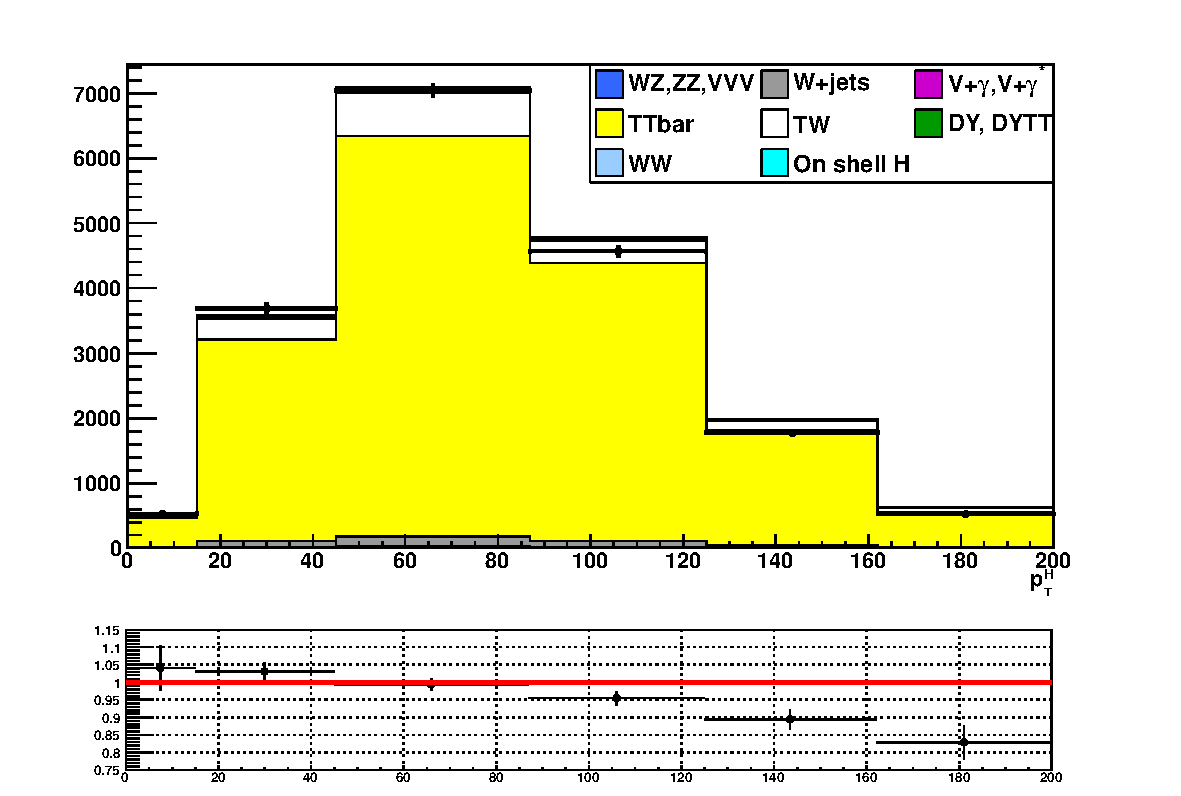
\includegraphics[width=0.6\textwidth]{images/ttpth.pdf}
\caption{Distribution of \pth in the $CR_{\ttbar}$ region, comparing data and simulation.\label{fig:ttpth}}
\end{figure}

The results of the method discussed before are listed in Tab.~\ref{tab:ttdd} for each bin of \pth.

\begin{table}[htb]
\caption{Data driven scale factors related to the top quark background estimation.\label{tab:ttdd}}
\centering
\begin{tabular}{c c c c c c}
\toprule
\pth [\GeV] & $N_\mathrm{Data}^{CR_{\ttbar}}$ & $N_\mathrm{MC}^{CR_{\ttbar}}$ &  $N_\mathrm{MC}^{SR}$ & $\alpha$ & $\Delta\alpha$ \\ 
\midrule
$[0 \textendash 15]$ & 406.7 & 358.8 & 117.8 & 0.33 & 0.08 \\ 
$[15 \textendash 45]$ & 2930.1 & 2703.4 & 859.1 & 0.32 & 0.07 \\ 
$[45 \textendash 85]$ & 5481.0 & 5207.5 & 1506.1 & 0.29 & 0.07 \\ 
$[85 \textendash 125]$ & 4126.4 & 4032.6 & 861.2 & 0.21 & 0.05 \\ 
$[125 \textendash 165]$ & 1612.6 & 1654.3 & 304.7 & 0.18 & 0.06 \\ 
$[165 \textendash \infty]$ & 647.5 & 760.4 & 201.7 & 0.27 & 0.15 \\ 
\bottomrule
\end{tabular}
\end{table}

A comparison of the \mll distributions in the $CR_{\ttbar}$ region for data and simulation is shown in Fig.~\ref{fig:mllCtrlDD}, separately for each \pth bin and after the application of the data-driven factors. The agreement between data and simulation is found to be satisfactory within uncertainties.

\begin{figure}[htb]
\centering
\subfigure[$\pth<15\GeV$]{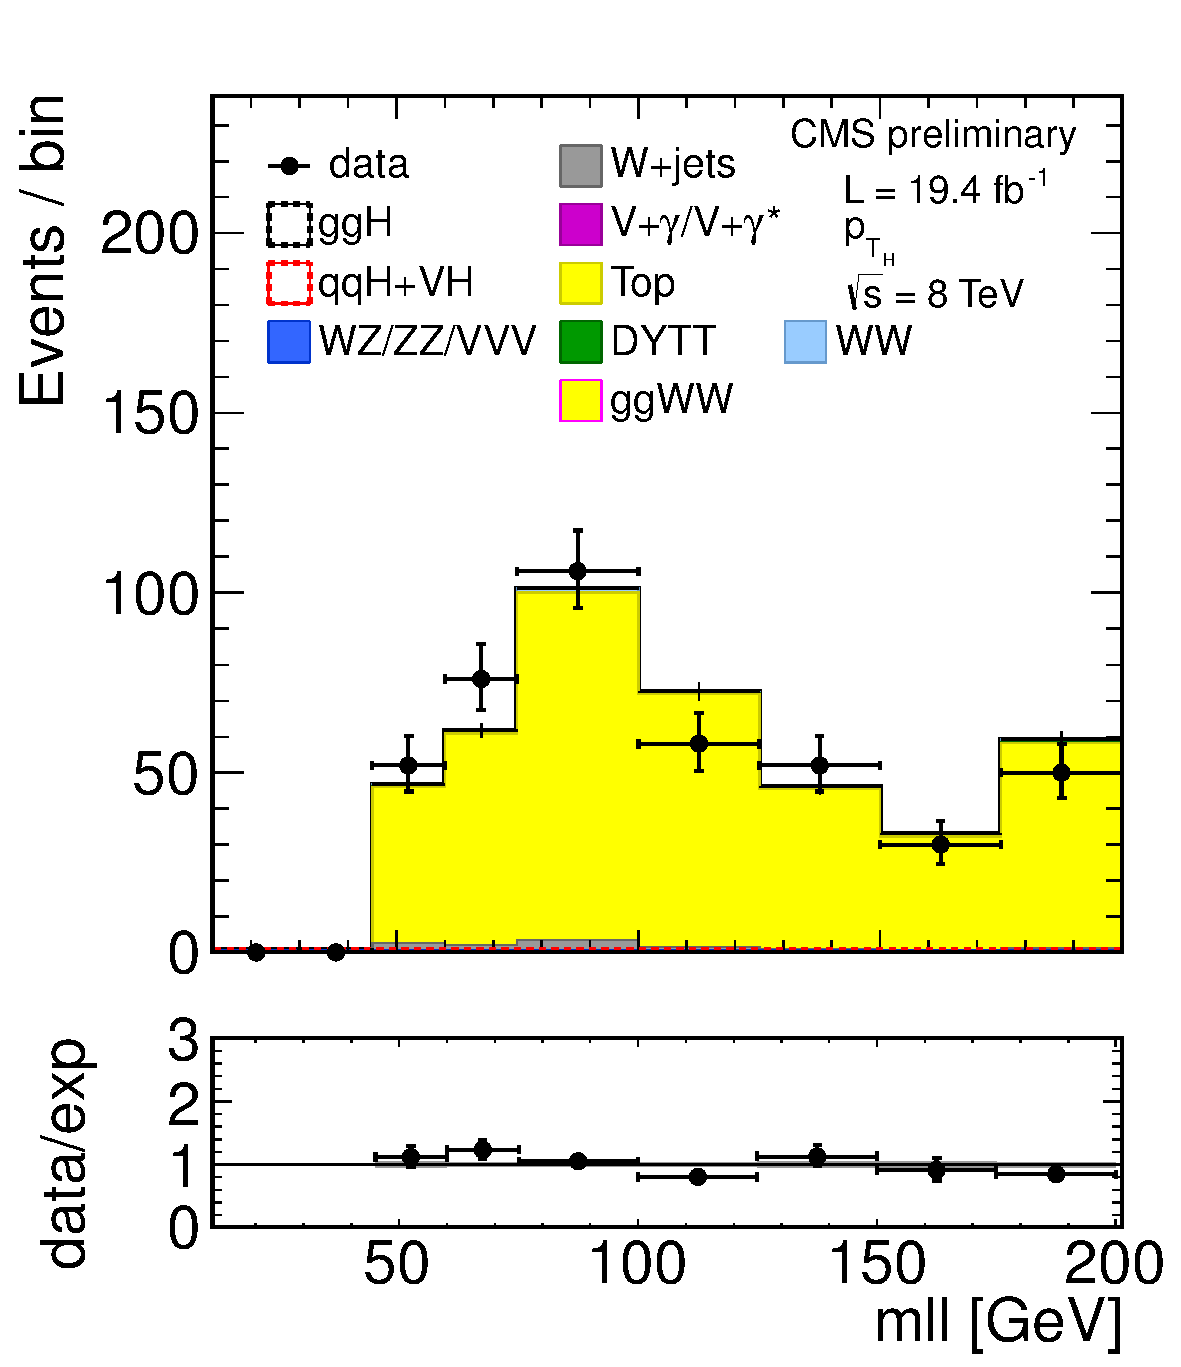
\includegraphics[width=0.31\textwidth]{images/mllBin0CtrlDD.pdf}}
\subfigure[$15\GeV<\pth<45\GeV$]{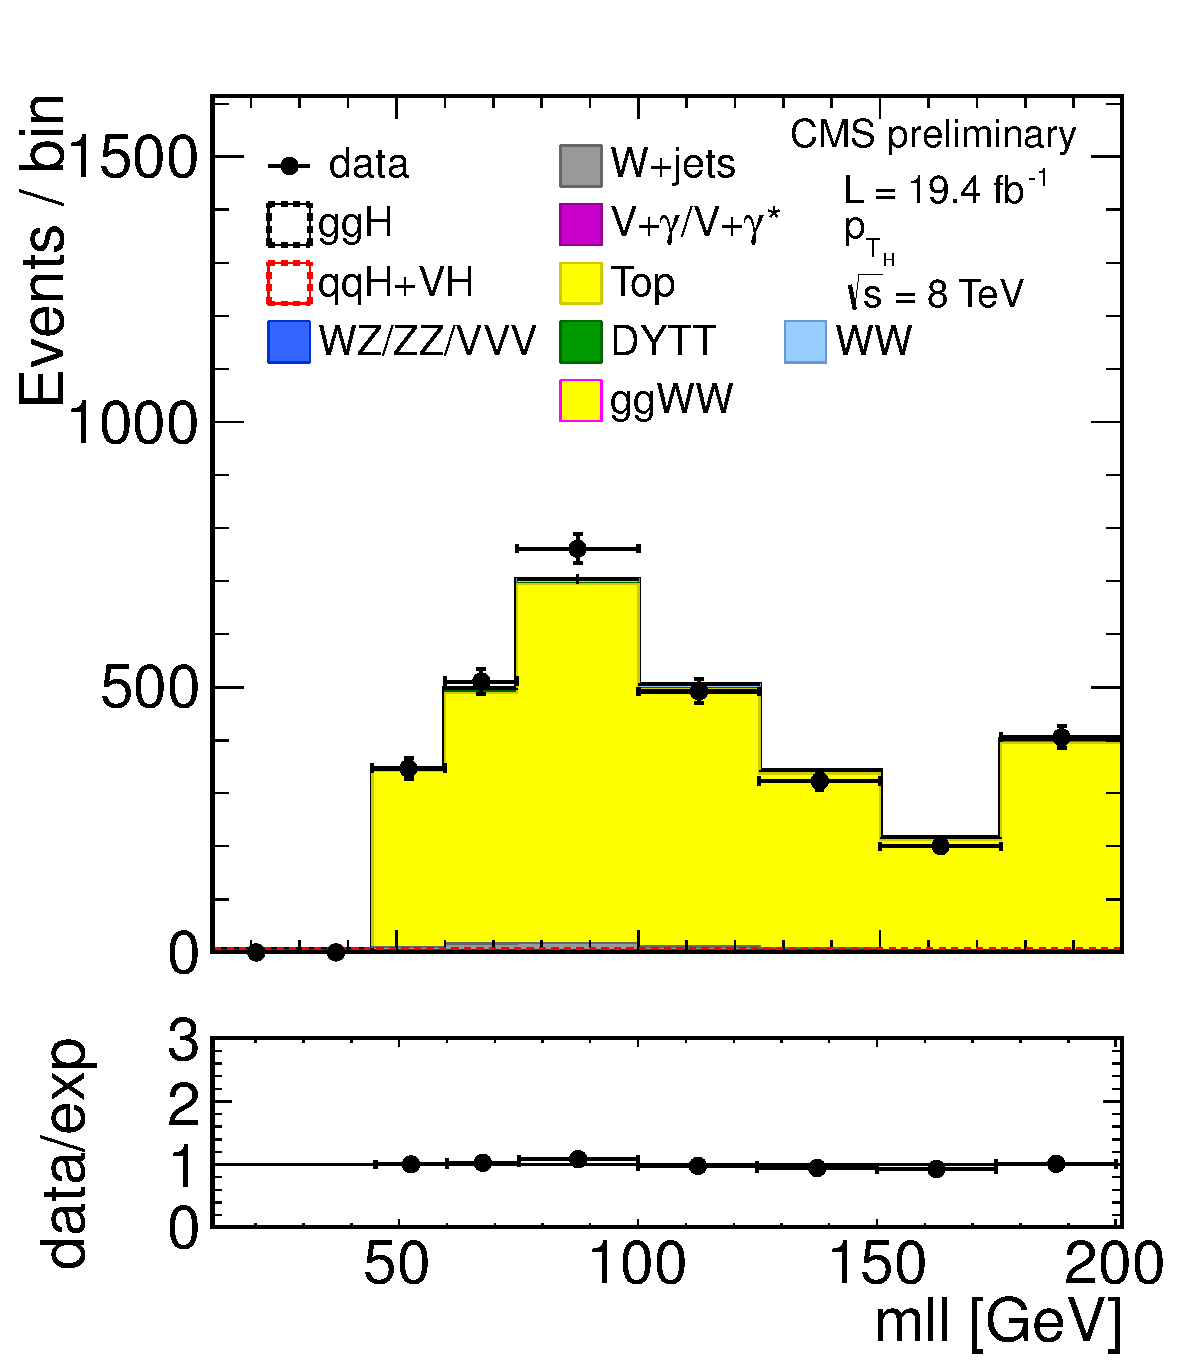
\includegraphics[width=0.31\textwidth]{images/mllBin1CtrlDD.pdf}}
\subfigure[$45\GeV<\pth<85\GeV$]{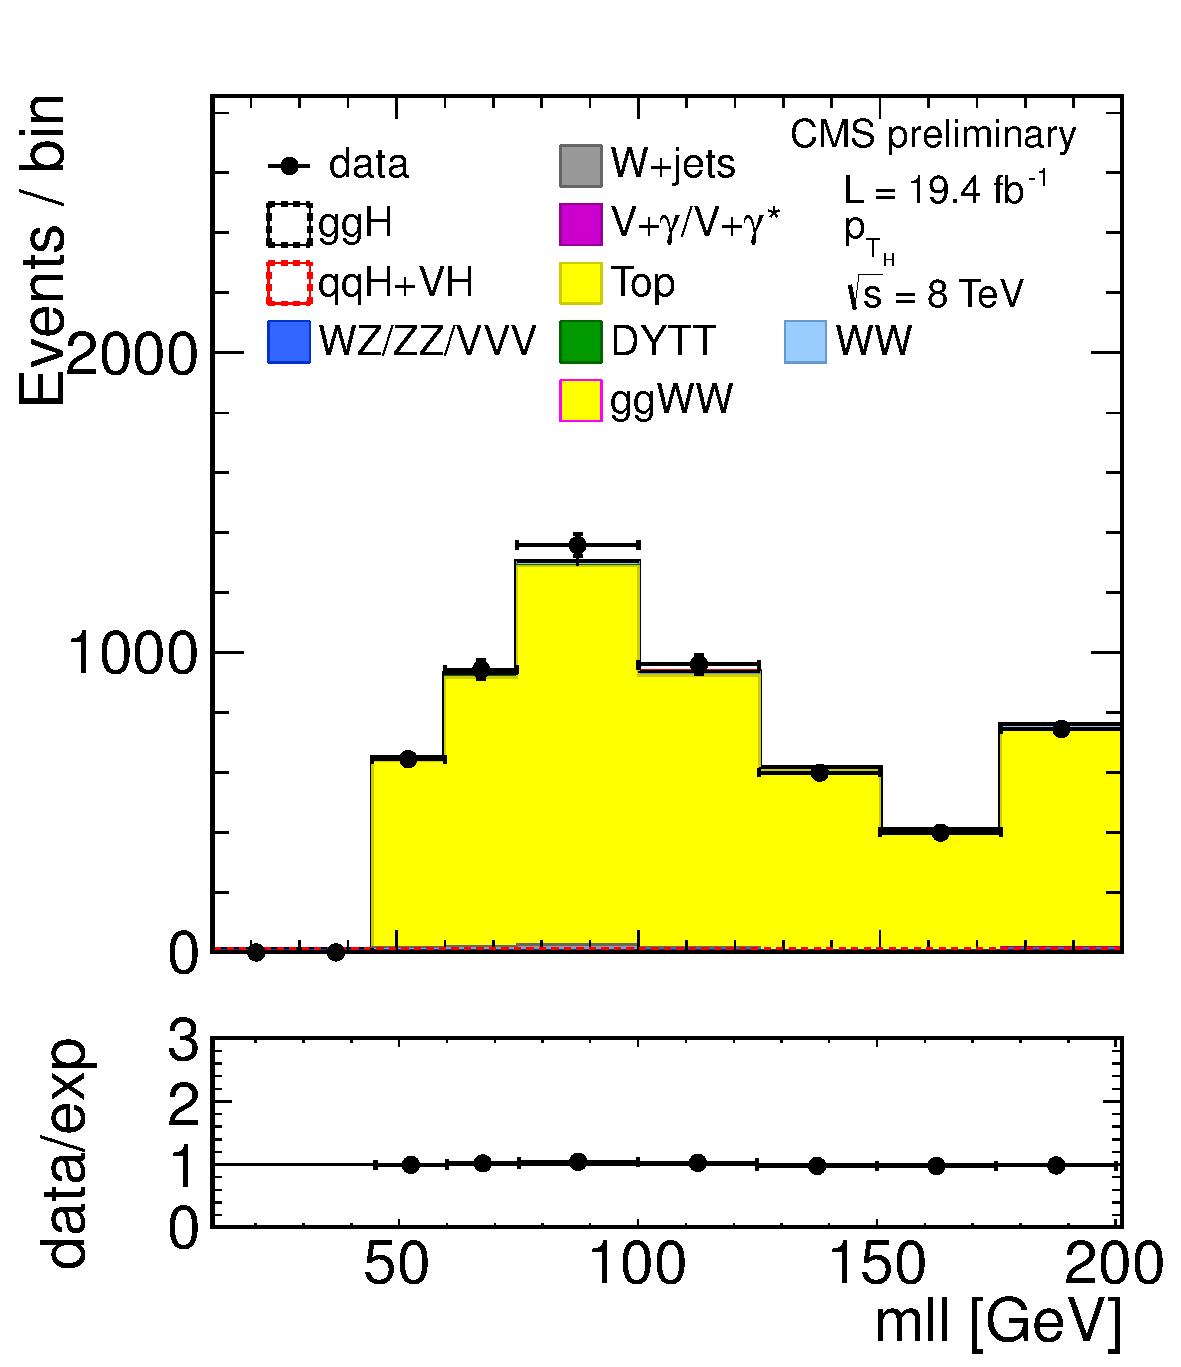
\includegraphics[width=0.31\textwidth]{images/mllBin2CtrlDD.pdf}}\\
\subfigure[$85\GeV<\pth<125\GeV$]{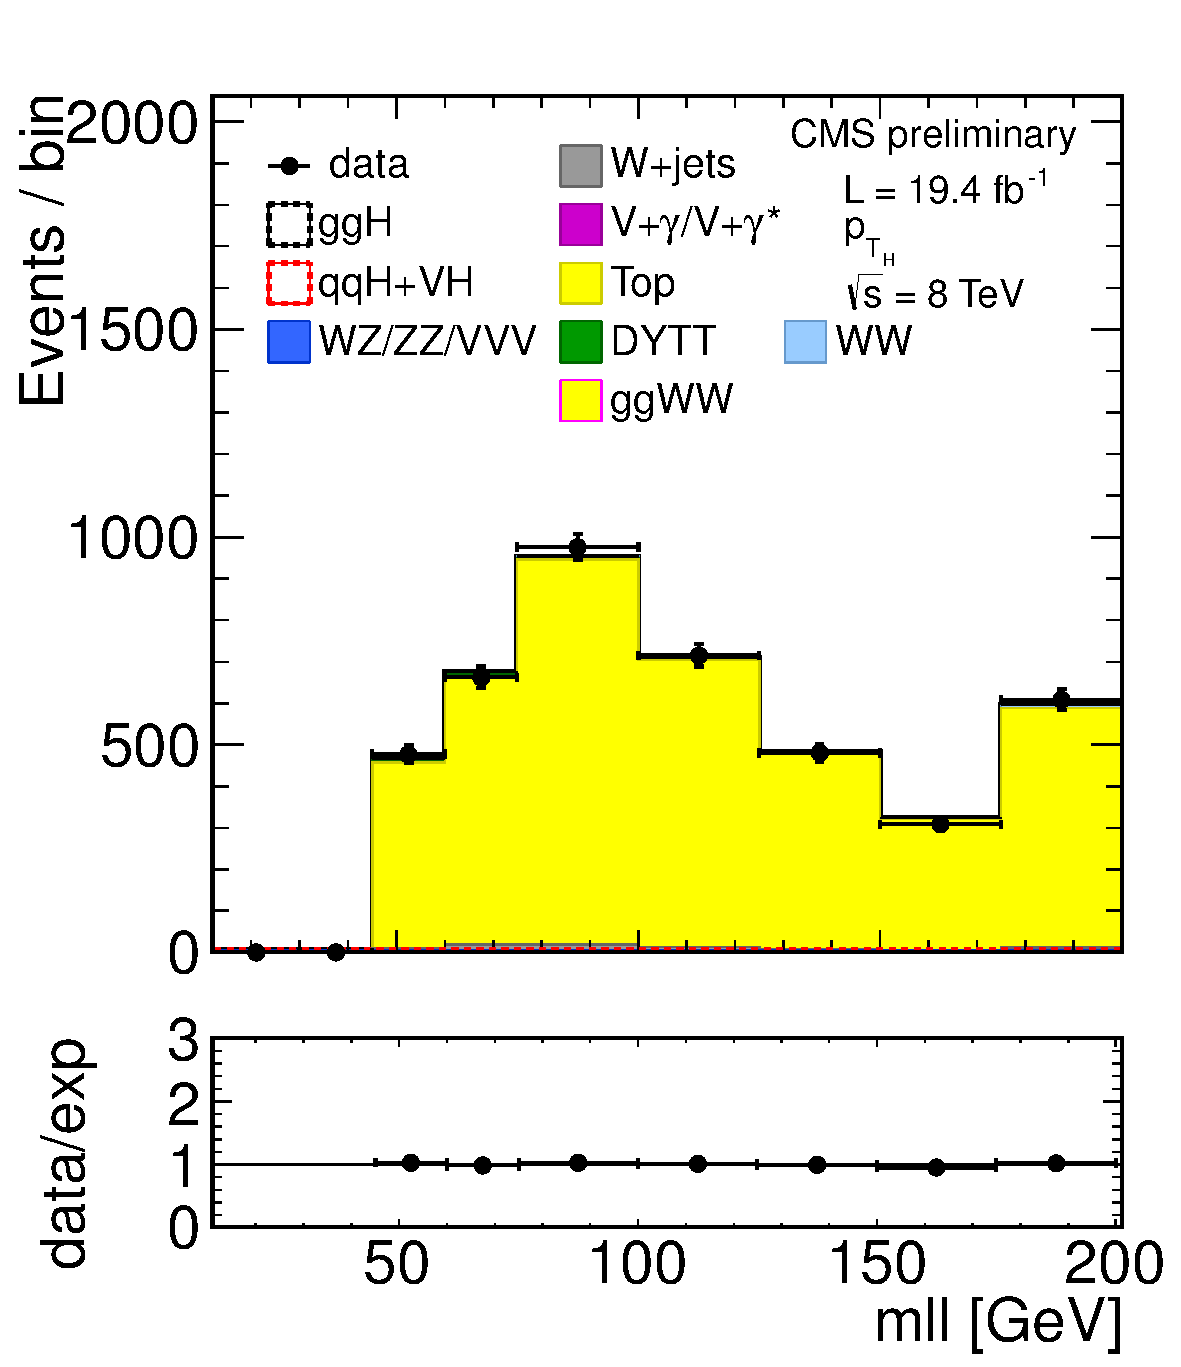
\includegraphics[width=0.31\textwidth]{images/mllBin3CtrlDD.pdf}}
\subfigure[$125\GeV<\pth<165\GeV$]{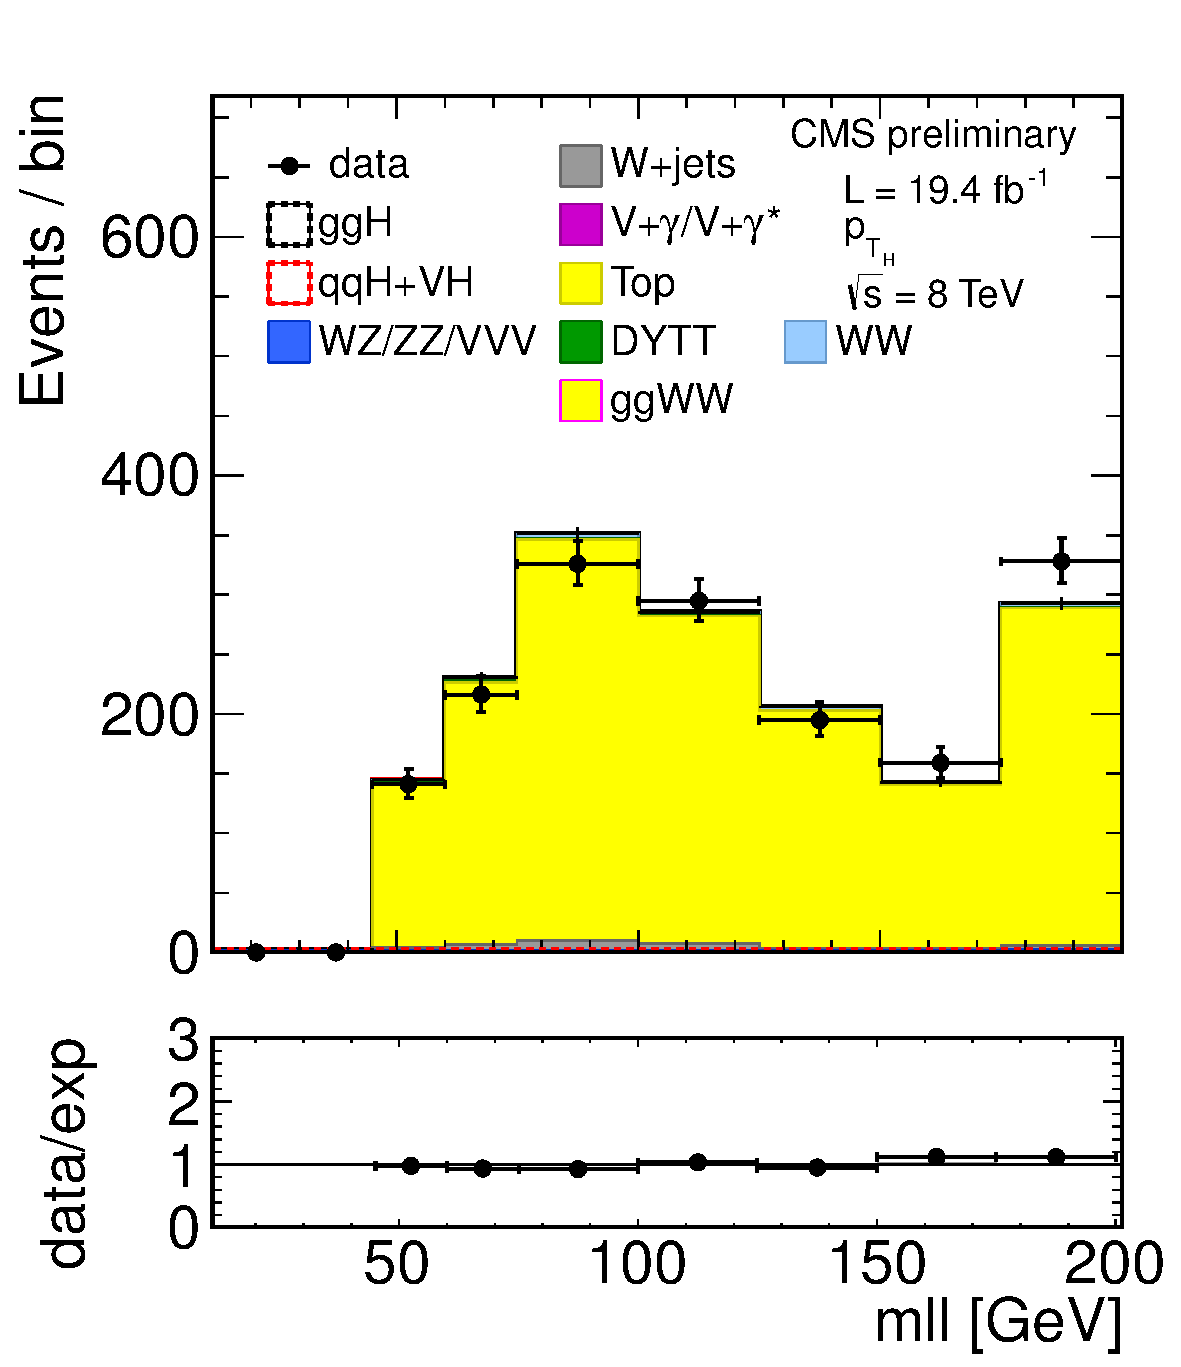
\includegraphics[width=0.31\textwidth]{images/mllBin4CtrlDD.pdf}}
\subfigure[$\pth>165\GeV$]{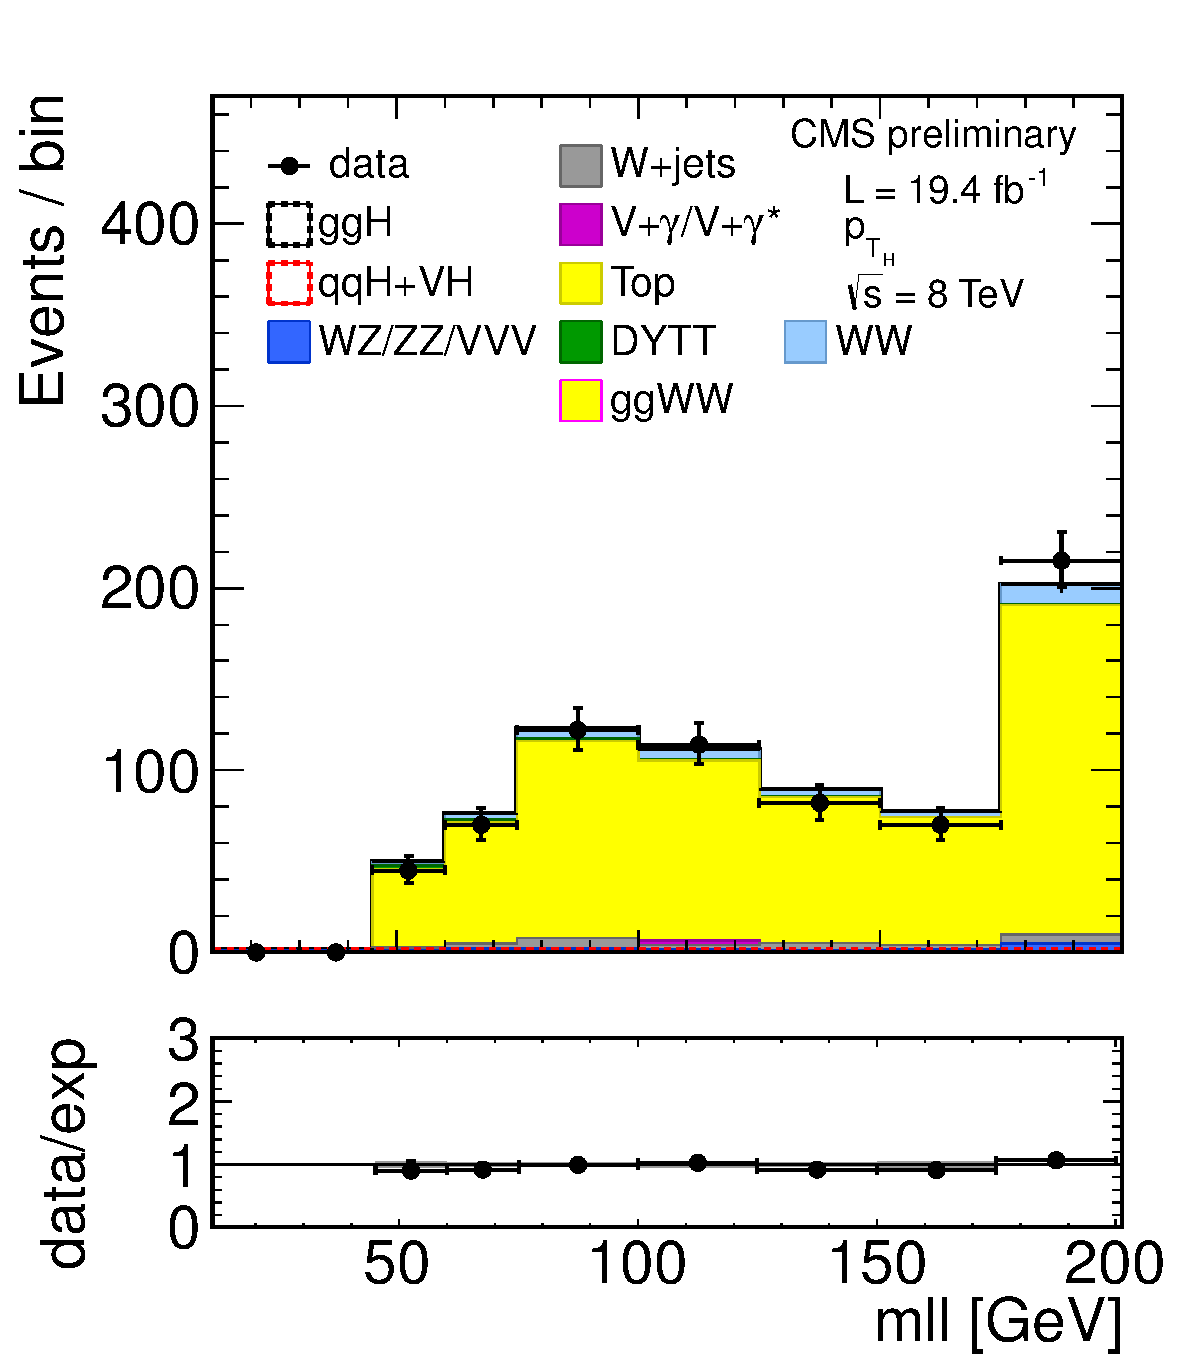
\includegraphics[width=0.31\textwidth]{images/mllBin5CtrlDD.pdf}}
\caption{Comparison of the \mll distributions in the $CR_{\ttbar}$ region for data and simulation in each \pth bin, after the application of the data-driven factors.\label{fig:mllCtrlDD}}
\end{figure}






\subsection{WW background \label{sec:WWBackground}}

First of all, the \mll and \mt shapes of the $\mathrm{qq\to W^{+}W^{-}}$ background process have been compared to the data in a signal free phase space, as shown in Fig.~\ref{fig:WW}. The signal-free region is defined requiring the preselections described in Sec.~\ref{sec:Selections} with the additional cut $\mll>70$\GeV. The comparison, which is performed inclusively in \pth in the 0 and 1 jet categories, shows a good data to simulation agreement within uncertainties.

\begin{figure}[!htb]
\centering
\subfigure[\mll{} -- 0 jets]{
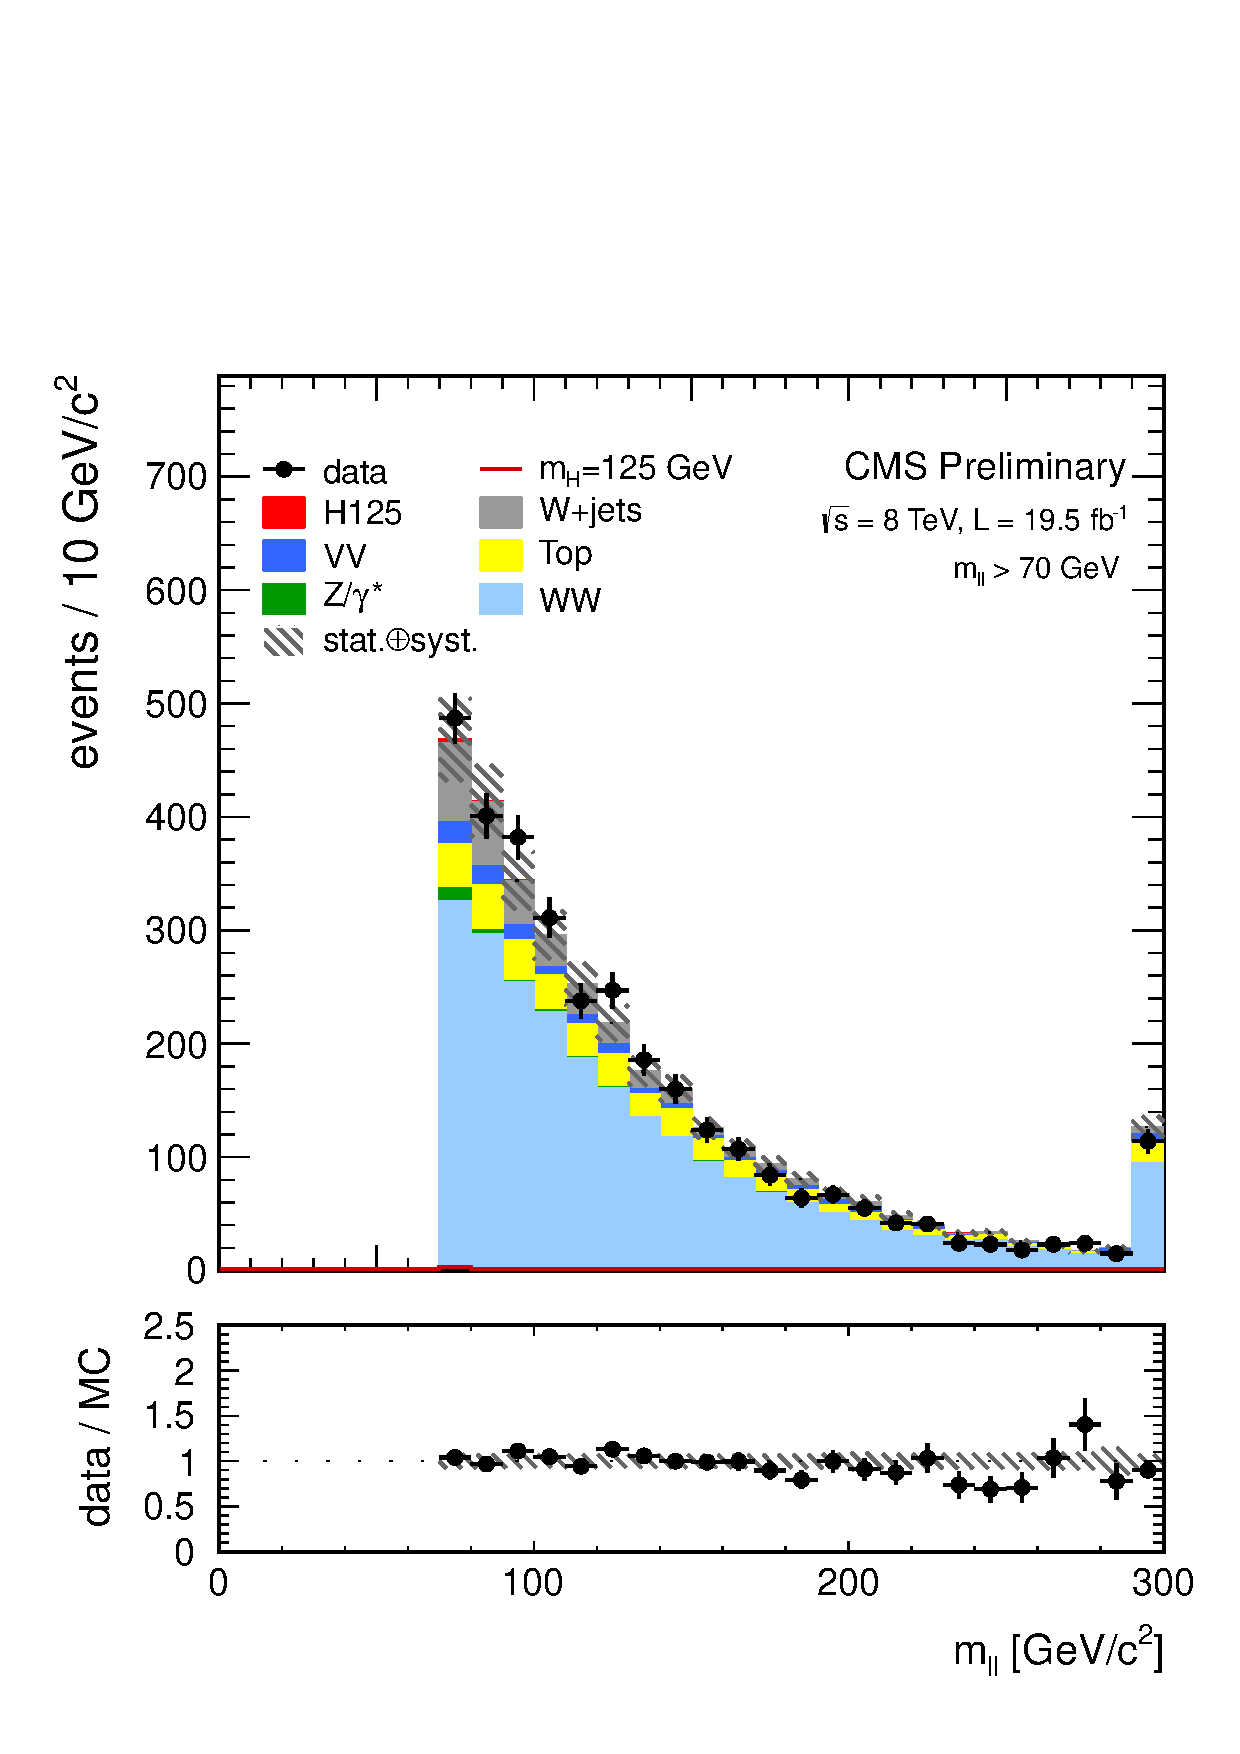
\includegraphics[width=0.35\textwidth]{images/WWctrl/mll0j.pdf}
}
\subfigure[\mt{} -- 0 jets]{
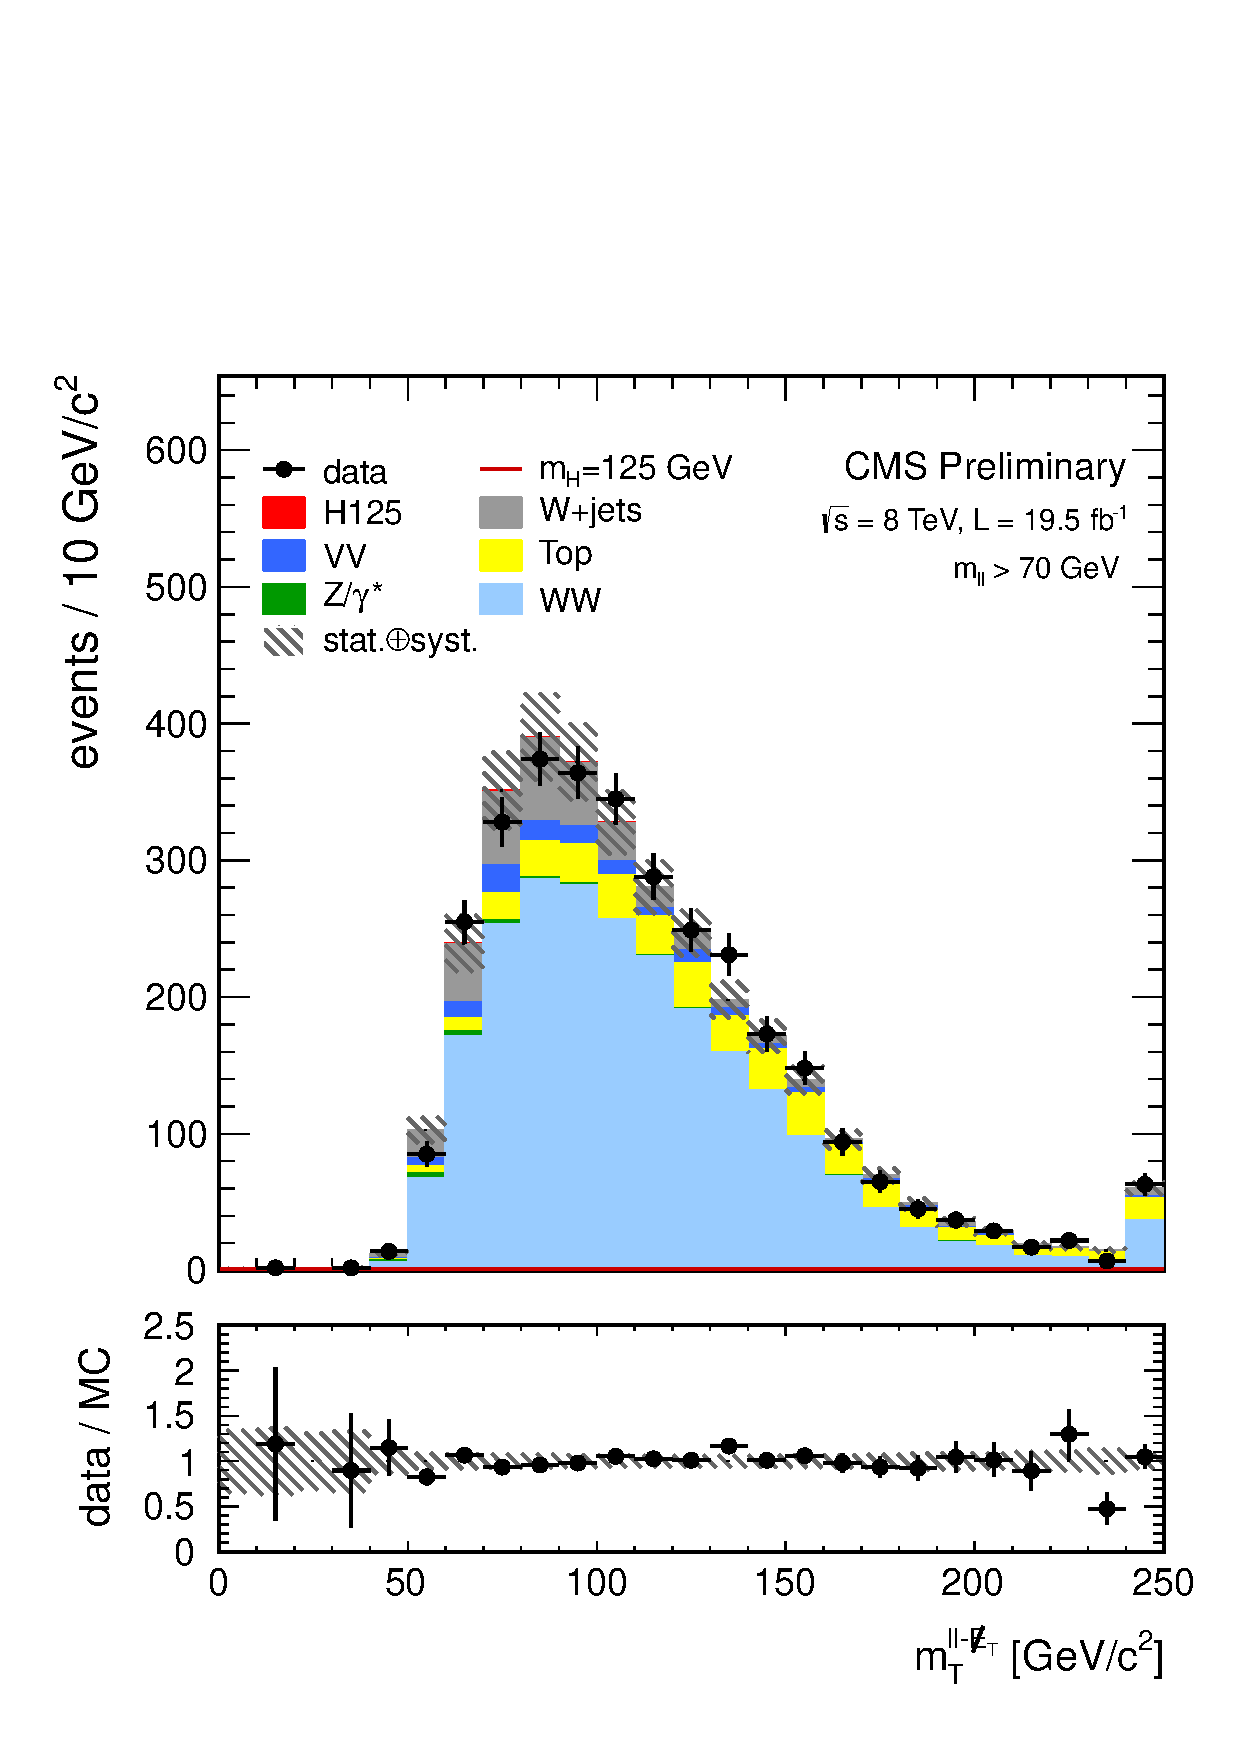
\includegraphics[width=0.35\textwidth]{images/WWctrl/mt0j.pdf}
}
\\
\subfigure[\mll{} -- 1 jet]{
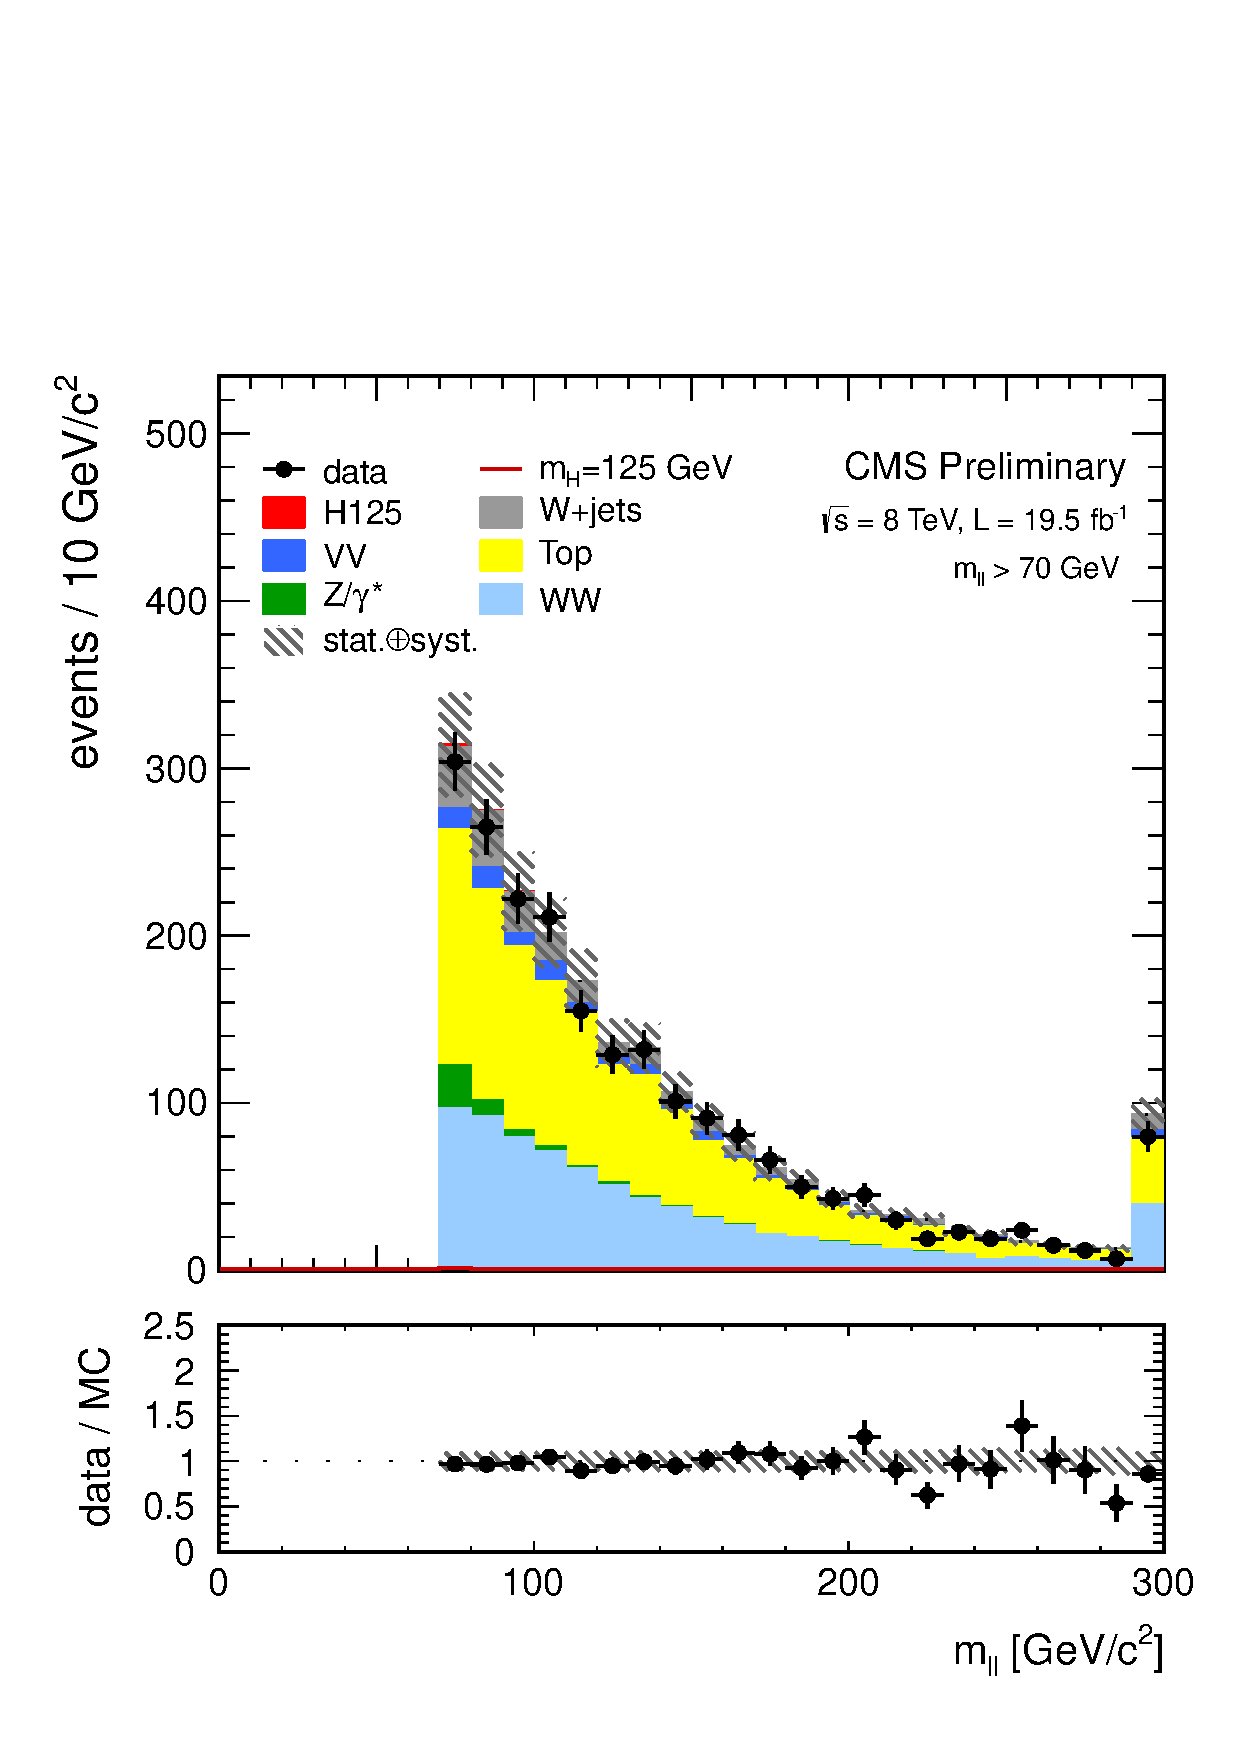
\includegraphics[width=0.35\textwidth]{images/WWctrl/mll1j.pdf}
}
\subfigure[\mt{} -- 1 jet]{
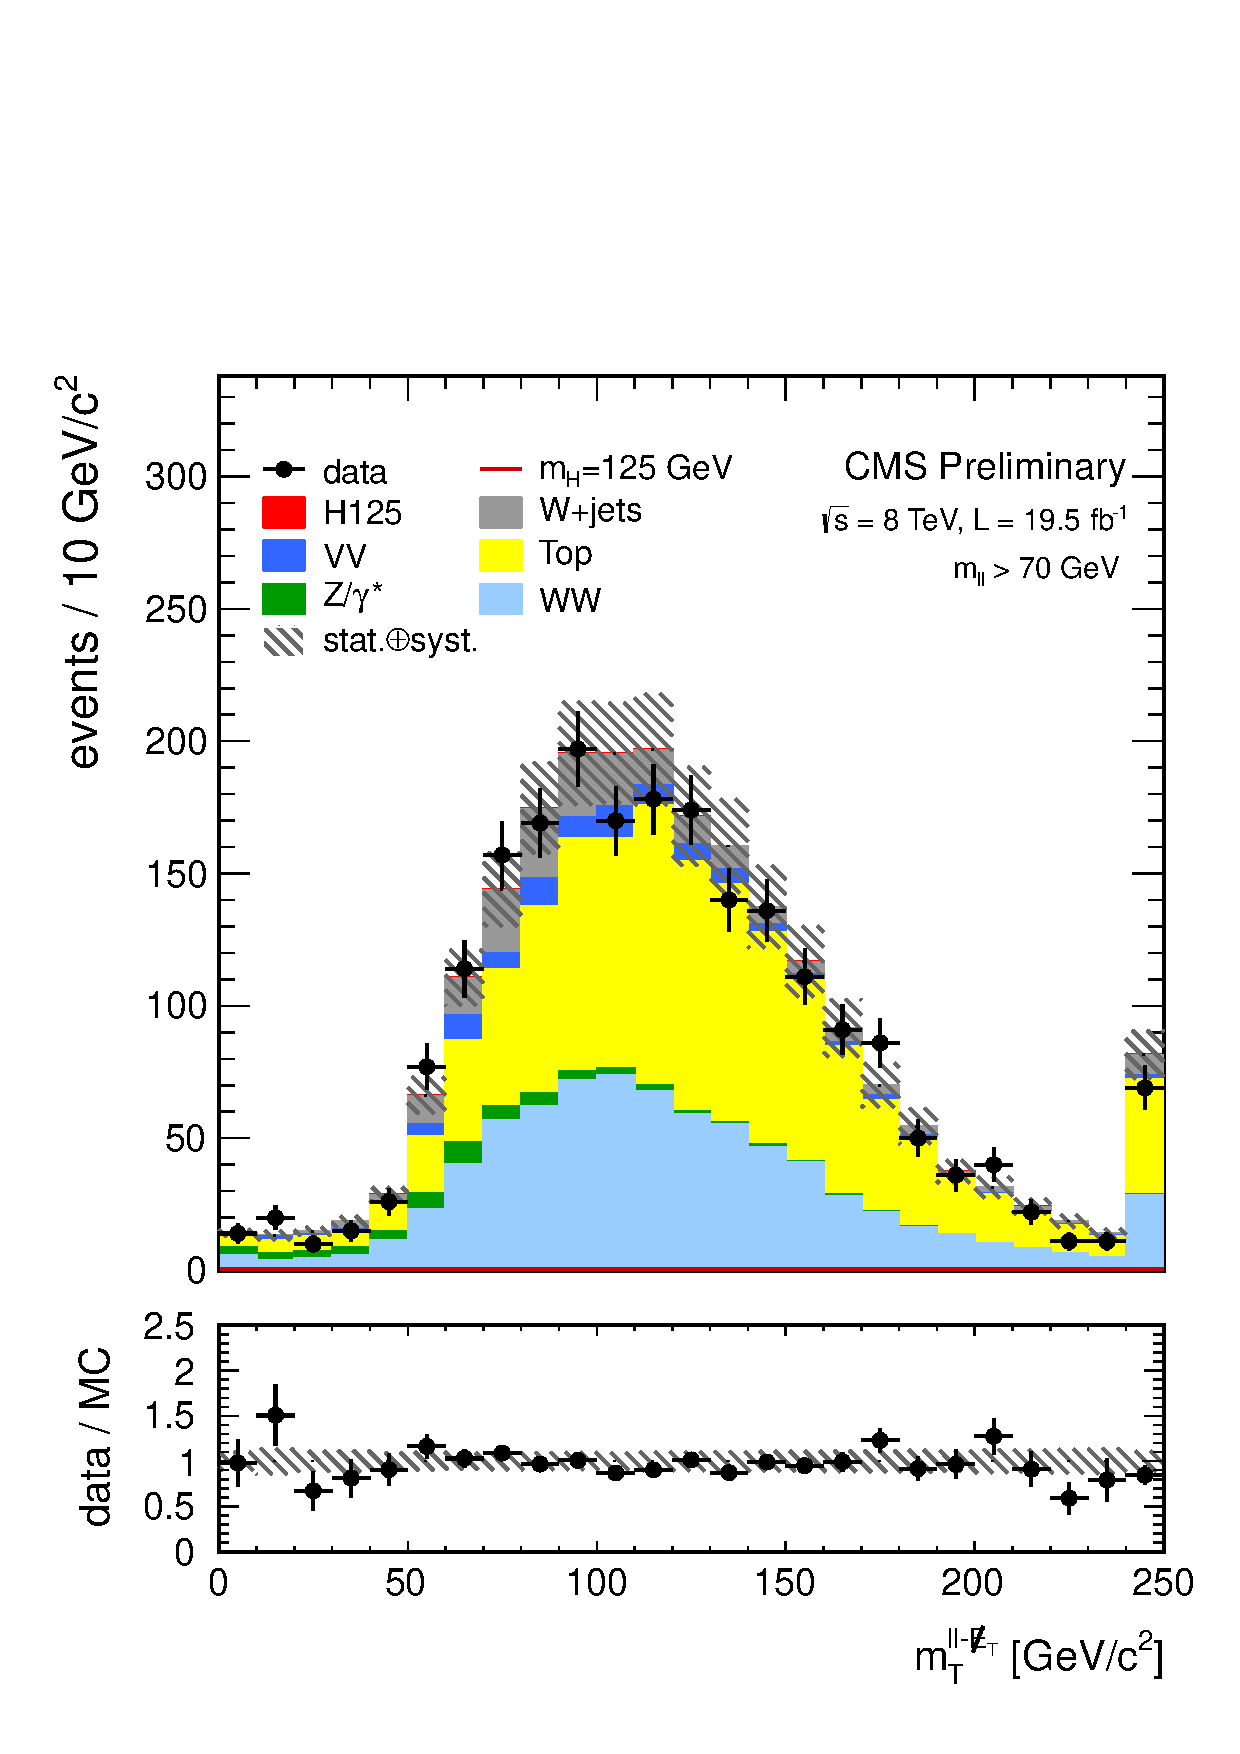
\includegraphics[width=0.35\textwidth]{images/WWctrl/mt1j.pdf}
}

\caption{Comparison of the \mll and \mt shapes in data and simulation for events with 0 and 1 jets, inclusive in \pth. The events are required to pass the analysis requirements and, in order to define a signal-free control region, to have $\mll > 70$\GeV.\label{fig:WW}}
\end{figure}

In this analysis the $\mathrm{qq\to W^{+}W^{-}}$ background normalization is left free to float in each of the six \pth bins to match the data during the fitting procedure. This choice helps mitigating the \pth shape difference between data and simulation. This difference is due to missing higher order QCD corrections in the adopted simulation, obtained using the \textsc{Madgraph} generator. In fact, as shown in Fig.~\ref{fig:ww_wwnlo}, the theoretical calculations for this process performed at NLO QCD accuracy and including soft-gluon resummation effects, i.e. NLO+NNLL accuracy, predict a rather different \pth spectrum.

\begin{figure}[htb]
\centering
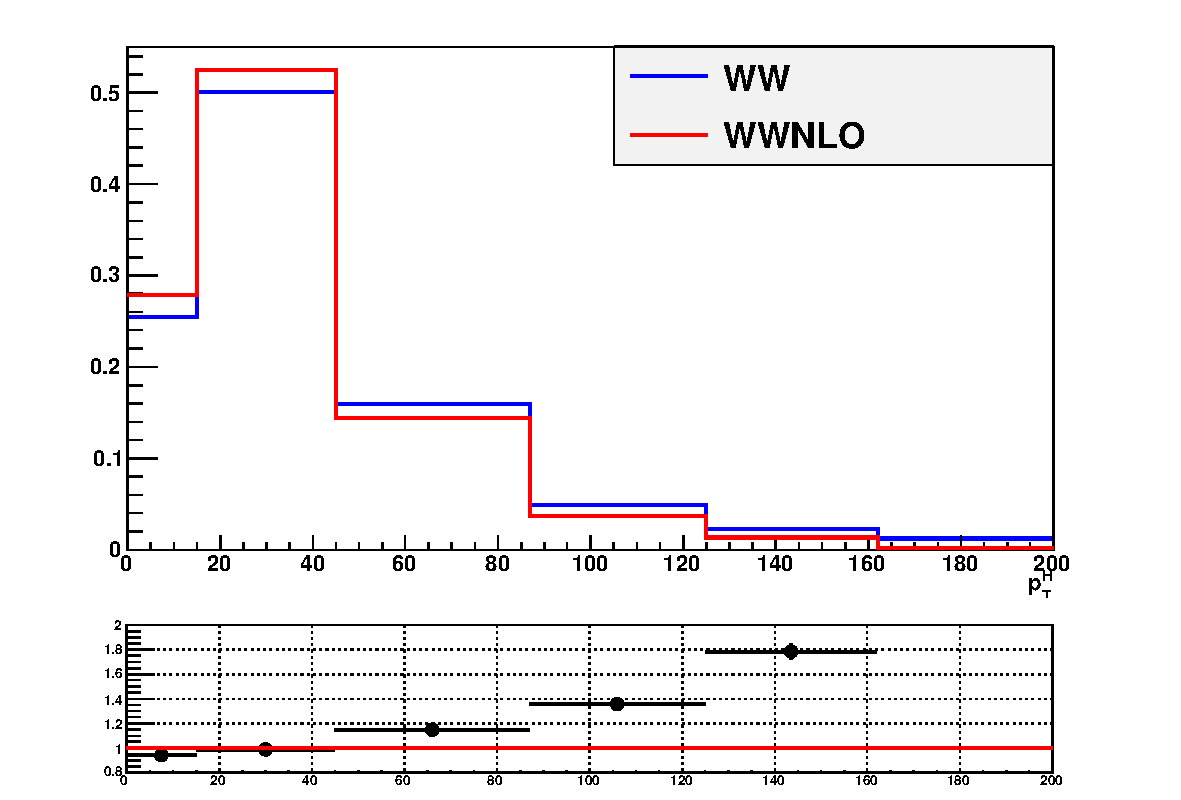
\includegraphics[width=0.6\textwidth]{images/WWnlo/WW_WWnlo.pdf}
\caption{Comparison between the $p_\mathrm{T}^\mathrm{WW}$ distributions obtained with two different MC generators: the blue line corresponds to the \textsc{Madgraph} generator and the red line refers to he same sample in which a reweighting has been applied in order to match the theoretical prediction at NLO+NNLL precision. }\label{fig:ww_wwnlo}
\end{figure}

To check the residual dependence of the \mll and \mt shapes on the generator used for simulating the $\mathrm{qq\to W^{+}W^{-}}$ process, the shapes obtained using different generators have been compared in each \pth bin, as shown in Figs.~\ref{fig:ww_mll} and \ref{fig:ww_mth}. The usage of different generators only mildly affect the \mll and \mt shapes. Nevertheless the observed differences are taken as shape uncertainties and propagated through the fit.

\begin{figure}[htb]
\centering
\subfigure[$0<\pth<15$\GeV]{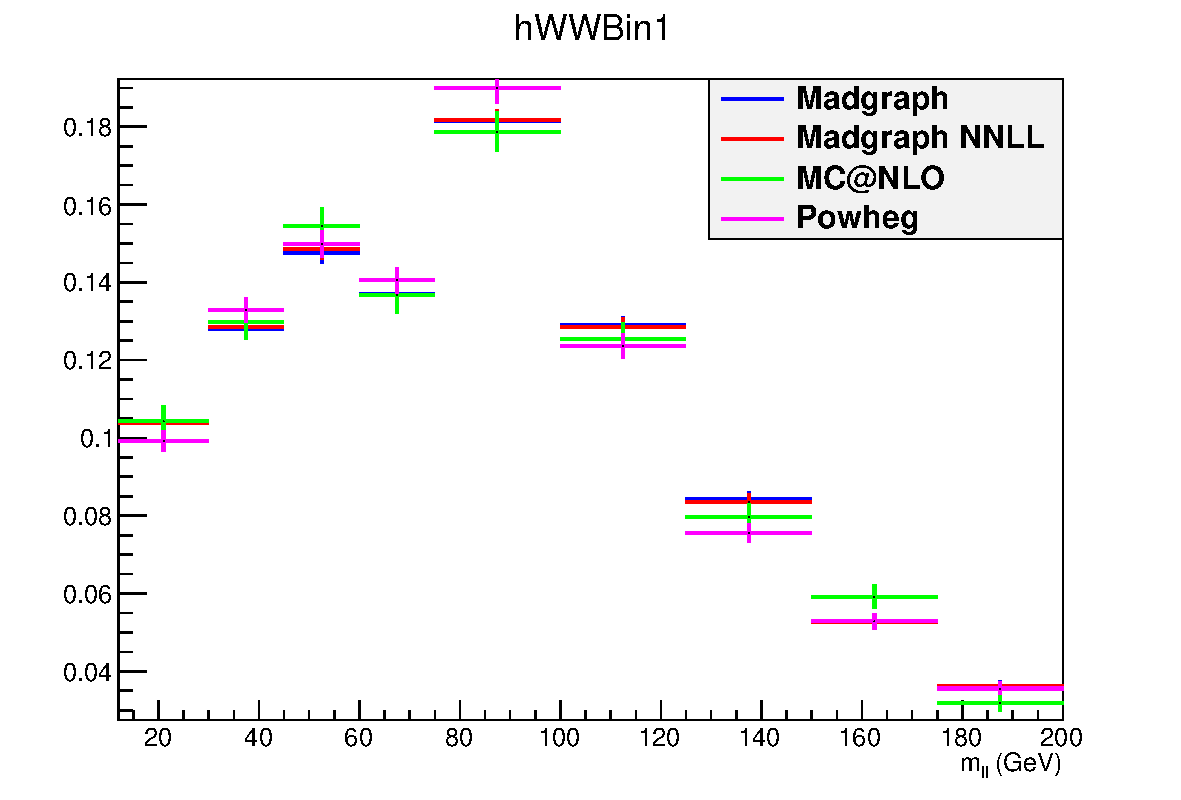
\includegraphics[width=0.31\textwidth]{images/WWnlo/mllBin1.pdf}}
\subfigure[$15<\pth<45$\GeV]{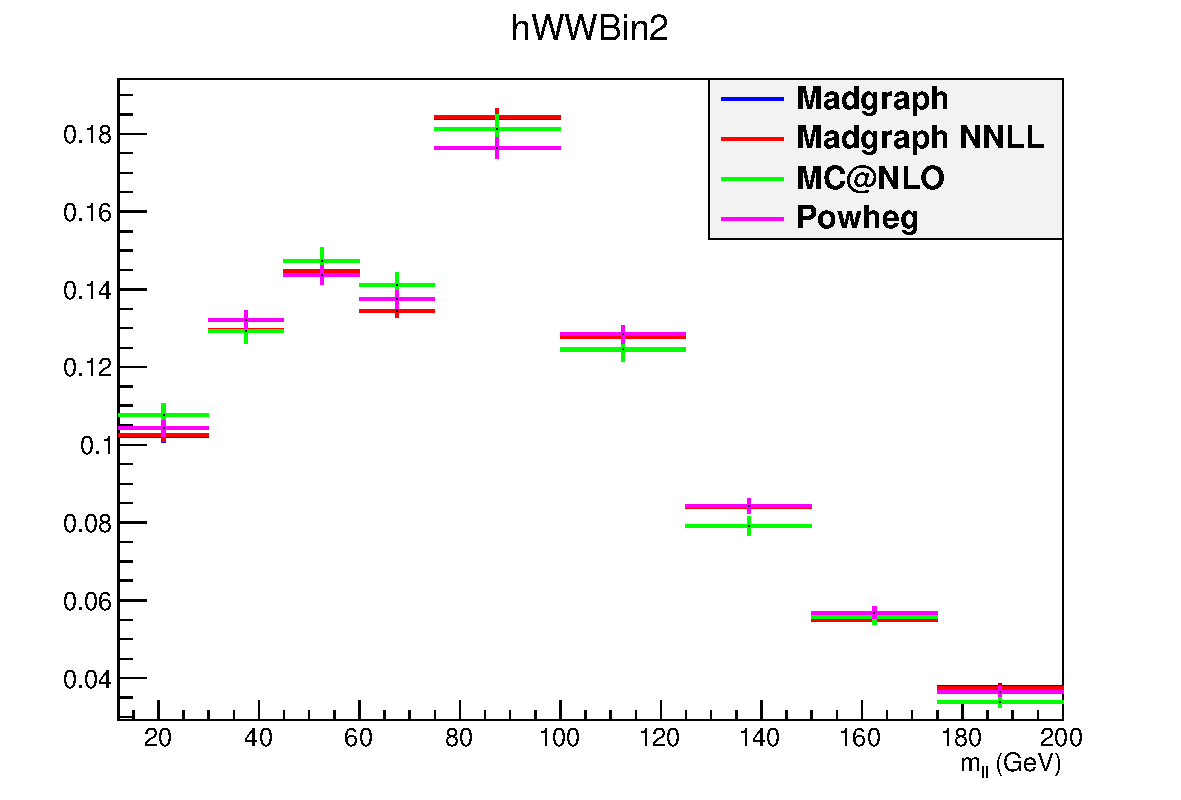
\includegraphics[width=0.31\textwidth]{images/WWnlo/mllBin2.pdf}}
\subfigure[$45<\pth<85$\GeV]{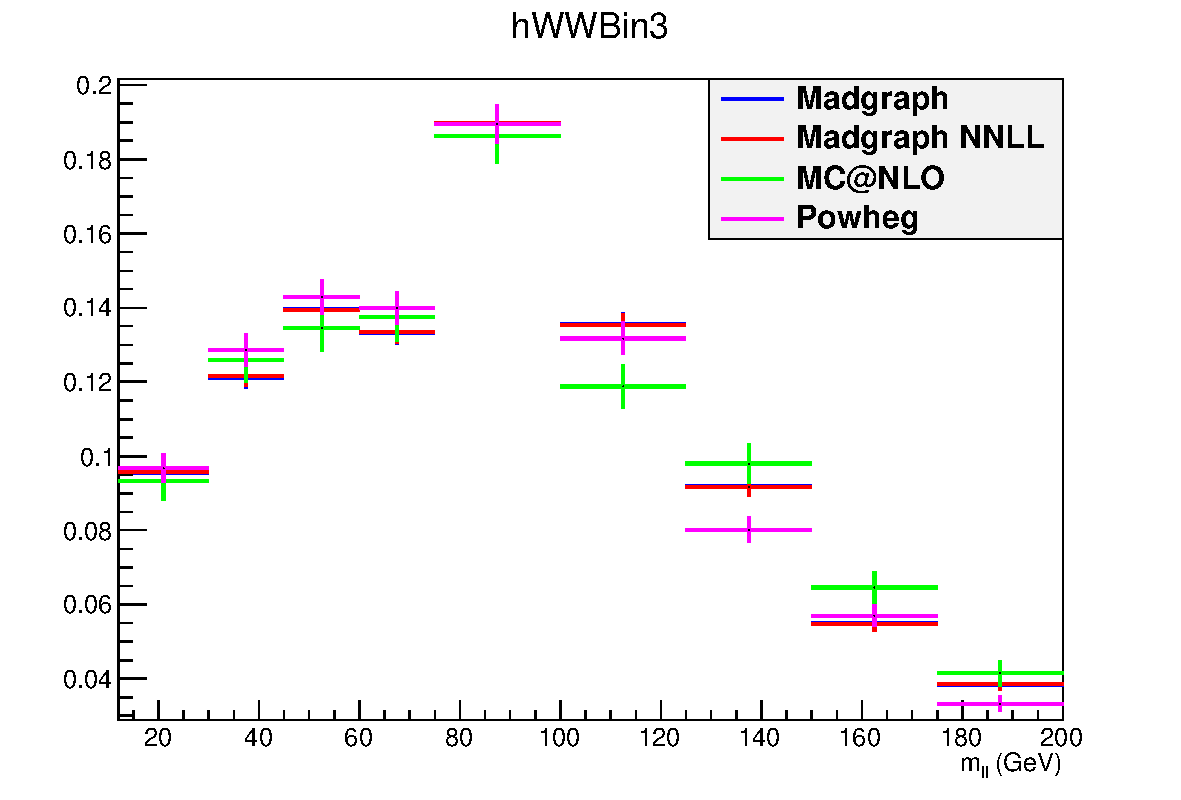
\includegraphics[width=0.31\textwidth]{images/WWnlo/mllBin3.pdf}}\\
\subfigure[$85<\pth<125$\GeV]{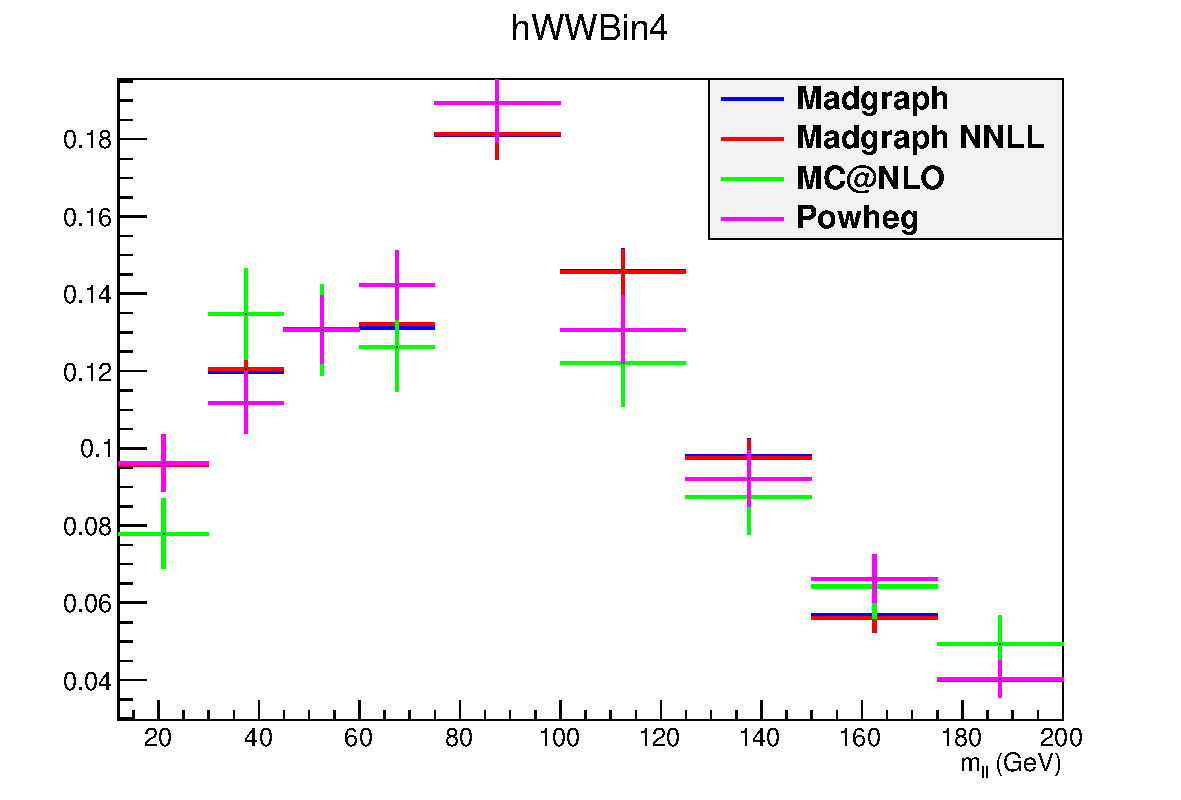
\includegraphics[width=0.31\textwidth]{images/WWnlo/mllBin4.pdf}}
\subfigure[$125<\pth<165$\GeV]{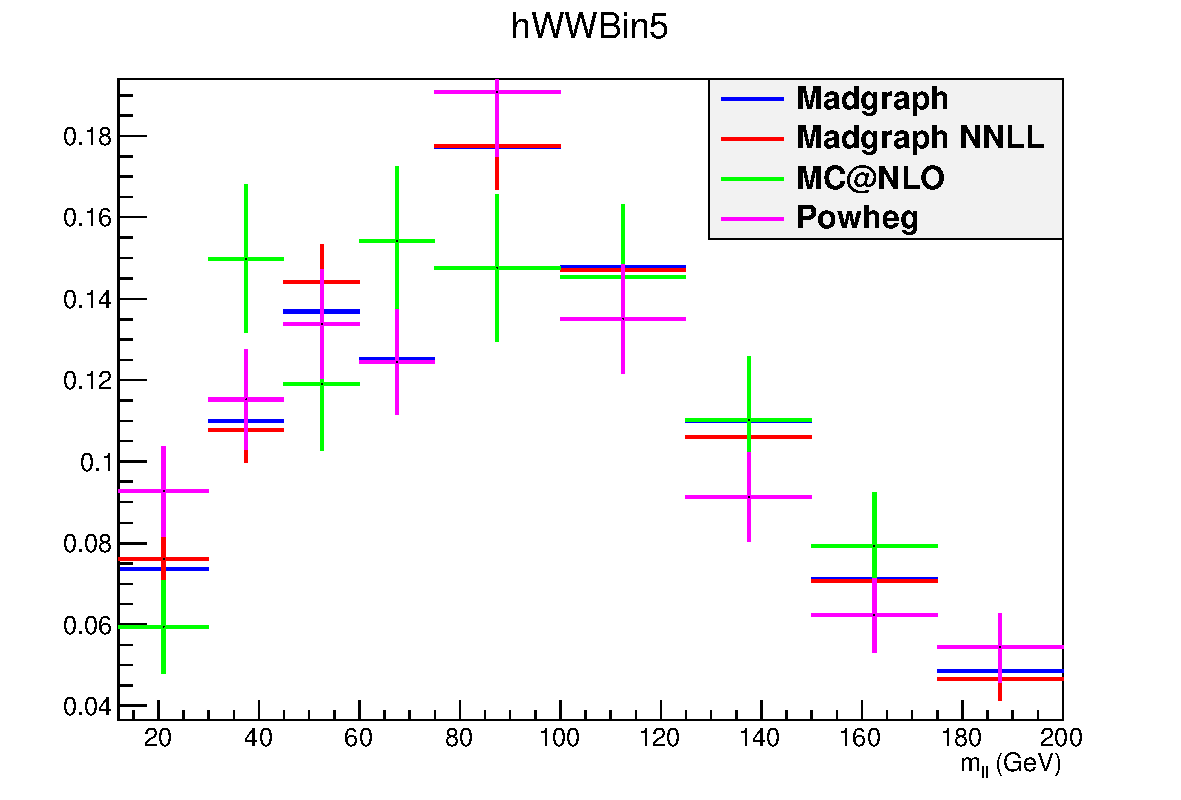
\includegraphics[width=0.31\textwidth]{images/WWnlo/mllBin5.pdf}}
\subfigure[$\pth>165$\GeV]{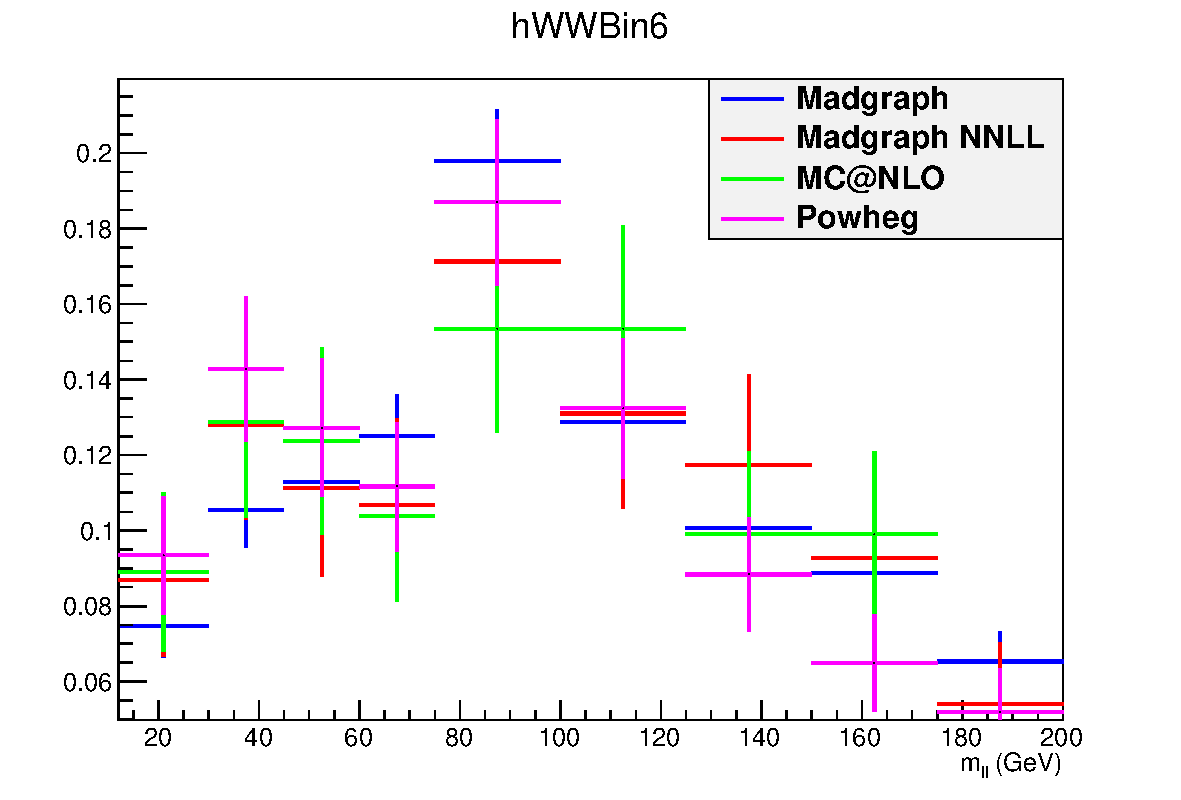
\includegraphics[width=0.31\textwidth]{images/WWnlo/mllBin6.pdf}}
\caption{Comparison between the \mll shape obtained with the default $\mathrm{qq\to W^{+}W^{-}}$ background simulation (\textsc{Madgraph}) and other theoretical models in every \pth bin.\label{fig:ww_mll}}
\end{figure}

\begin{figure}[htb]
\centering
\subfigure[$0<\pth<15$\GeV]{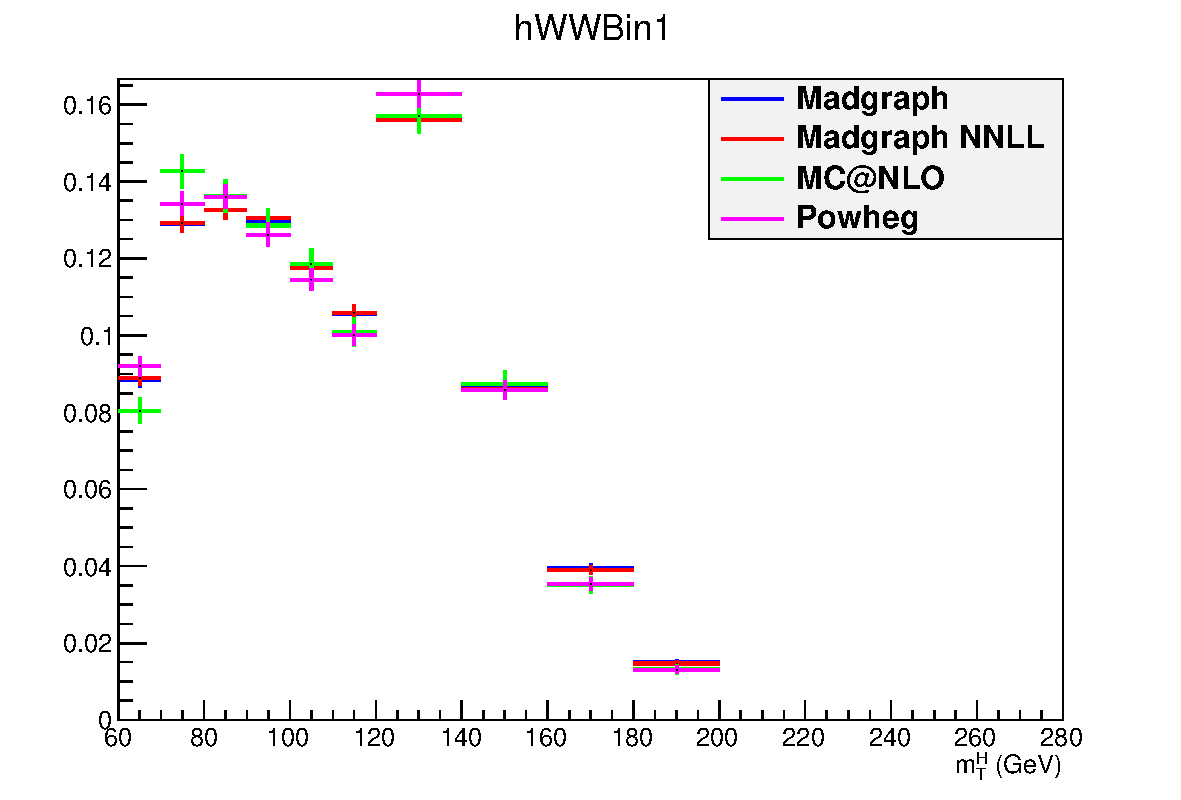
\includegraphics[width=0.31\textwidth]{images/WWnlo/mthBin1.pdf}}
\subfigure[$15<\pth<45$\GeV]{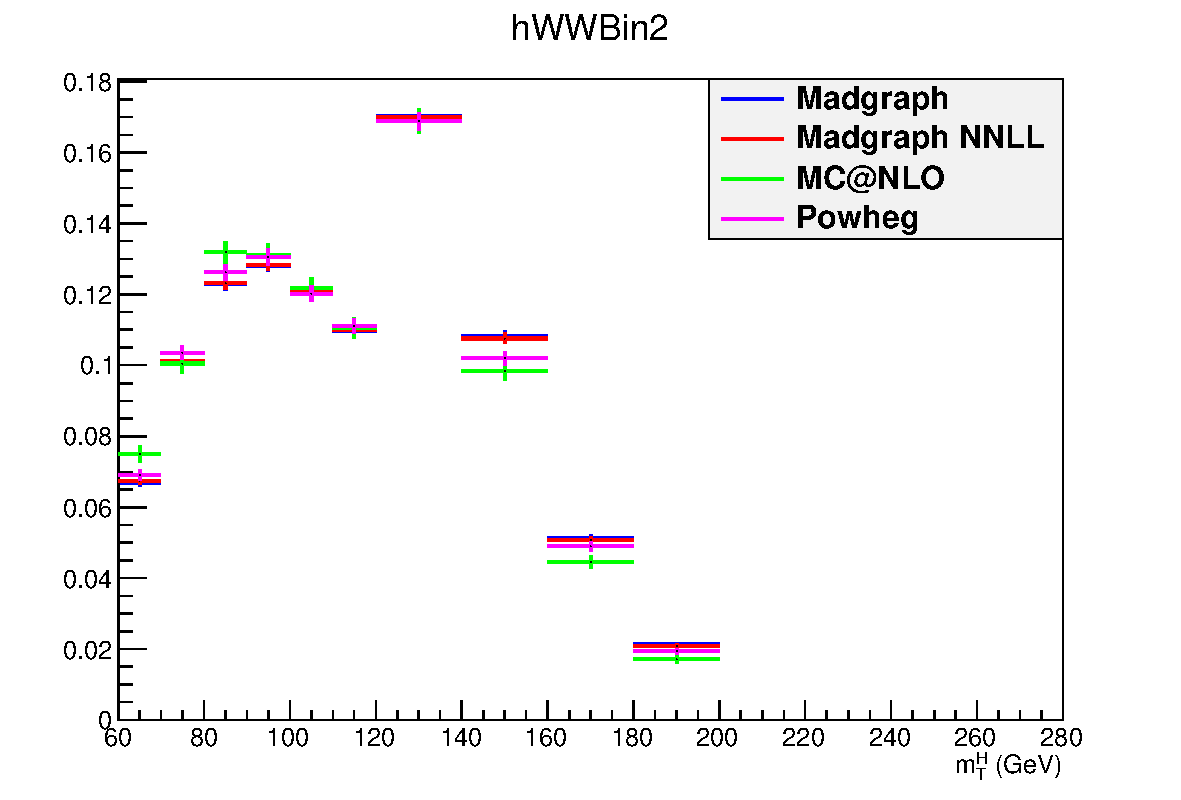
\includegraphics[width=0.31\textwidth]{images/WWnlo/mthBin2.pdf}}
\subfigure[$45<\pth<85$\GeV]{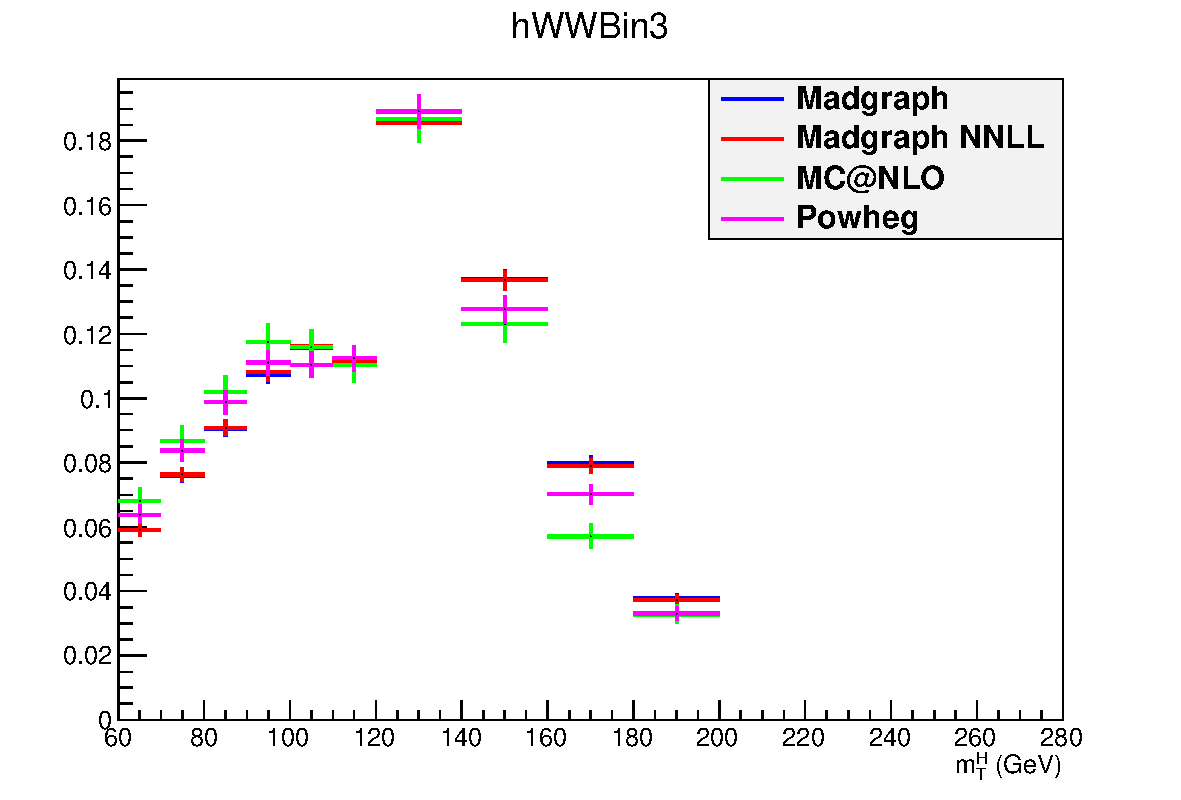
\includegraphics[width=0.31\textwidth]{images/WWnlo/mthBin3.pdf}}\\
\subfigure[$85<\pth<125$\GeV]{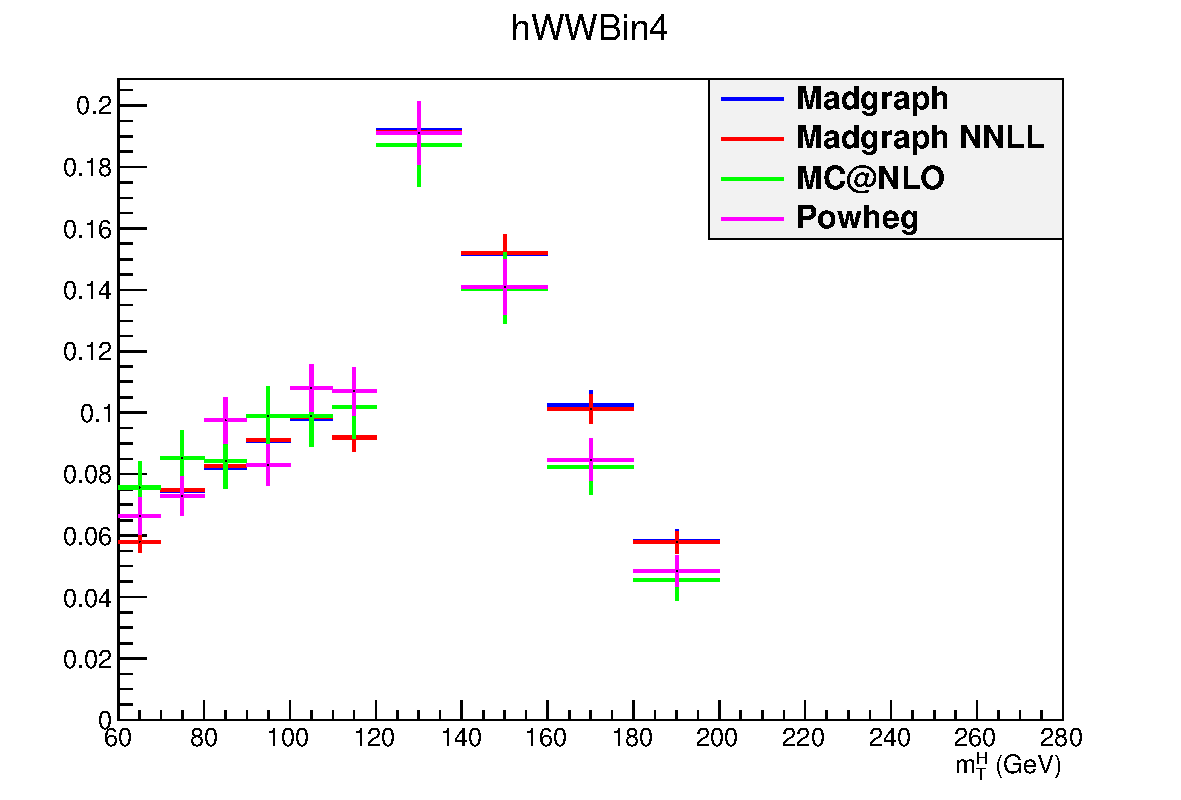
\includegraphics[width=0.31\textwidth]{images/WWnlo/mthBin4.pdf}}
\subfigure[$125<\pth<165$\GeV]{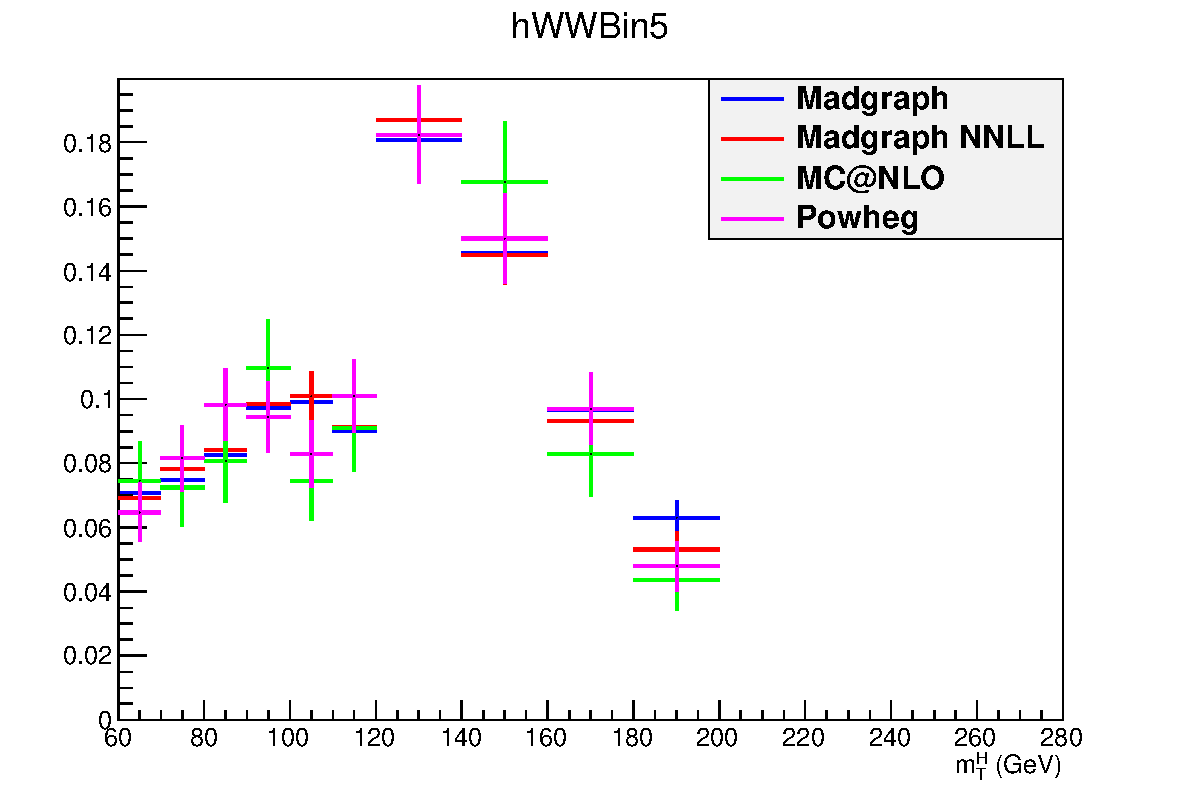
\includegraphics[width=0.31\textwidth]{images/WWnlo/mthBin5.pdf}}
\subfigure[$\pth>165$\GeV]{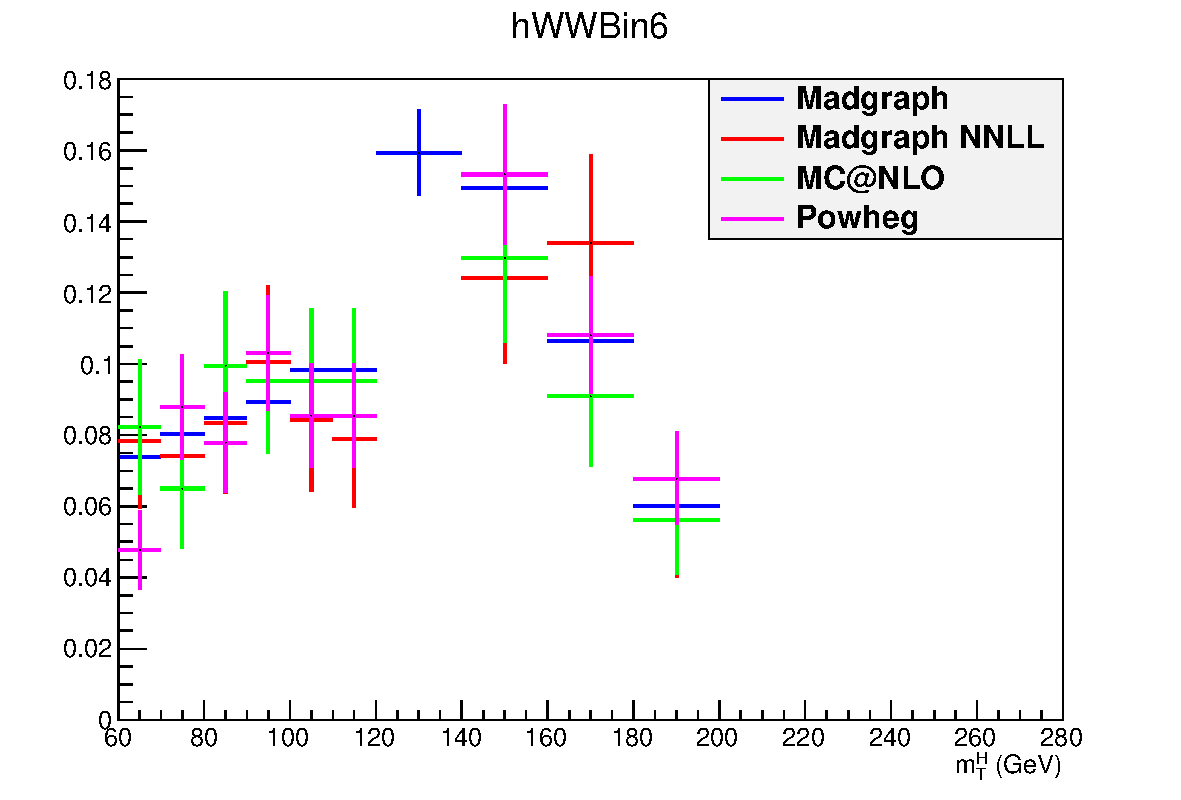
\includegraphics[width=0.31\textwidth]{images/WWnlo/mthBin6.pdf}}
\caption{Comparison between the \mt shape obtained with the default $\mathrm{qq\to W^{+}W^{-}}$ background simulation (\textsc{Madgraph}) and other theoretical models in every \pth bin.\label{fig:ww_mth}}
\end{figure}

The gluon-induced WW process, i.e. gg$\to \mathrm{W^{+}W^{-}}$, has a sub-dominant contribution with respect to the quark-induced process, being the cross section ratio between the two of about 5\%. The \mll and \mt shapes for this background are taken from simulation while the cross section is scaled to the approximate NLO calculation~\cite{Bonvini:2013jha,Passarino:2013bha}.




\subsection{W+jets background\label{sec:wjetsbkg}}	

The non-prompt lepton background, originating from leptonic decays of heavy quarks, hadrons
misidentified as leptons, and electrons from photon conversions in W+jets and QCD multijet production, is suppressed by the identification and isolation requirements on electrons and muons,  as described in Sec.~\ref{sec:leptonID}. The remaining contribution from the non-prompt lepton background is estimated directly from data and is ascribable especially to W+jets production. A control sample is defined by one lepton that passes the standard lepton selection criteria and another lepton candidate that fails the criteria, but passes a looser selection, resulting in a sample of ``pass-fail'' lepton pairs. 

The efficiency, $\varepsilon_\mathrm{pass}$, for a jet that satisfies the loose lepton requirements to pass the standard selection is determined using an independent sample dominated by events with non-prompt leptons from QCD multijet processes. However, this sample is not a pure sample containing just non-prompt leptons, but may still contain prompt leptons coming from the W and Z boson decays. To reject muons from the W decay, the events are required to have $\MET<20$\GeV and a W transverse mass below 20\GeV as well. Muons from the Z decay are instead removed requiring $m_{\mu\mu} \notin [76,106]$\GeV. For electrons the Z mass peak veto is enlarged to $m_\mathrm{ee} \notin [60,120]$\GeV. Finally, prompt electrons and muons are required to be isolated from the leading jet in the event, i.e. $\Delta\phi(\ell,j)>1$. The residual prompt lepton contamination from EW processes such as W/Z+jets production, which can bias the fake rate measurement, is estimated using simulation and subtracted. This contribution is negligible for small values of the lepton \pt and increases at larger \pt values.

The $\varepsilon_\mathrm{pass}$ efficiency, parametrized as a function of \pt and $\eta$ of the lepton, is then used to weight the events in the pass-fail sample by $\varepsilon_\mathrm{pass}/(1-\varepsilon_\mathrm{pass})$, to obtain the estimated contribution from the non-prompt lepton background in the signal region. The systematic uncertainties from the determination of $\varepsilon_\mathrm{pass}$ dominate the overall uncertainty of this method.

A validation of the estimate of this background is performed in a control sample obtained selecting events with two leptons with same charge, which is enriched in W+jets events. The results of this closure test show good agreement between data and the estimated background.

\begin{comment}
The idea is to estimate the background containing one or two fake leptons selecting events with relaxed lepton quality criteria, i.e. looser with respect to the selections used at the analysis level, and computing the efficiencies for real and fake leptons to pass the tight lepton quality requirements of the analysis. 
A data-driven approach is pursued to estimate this background. A set of loosely selected lepton-like objects, referred to as the ``fakeable object' or ``denominator'' from here on, is defined in a data set of events dominated by dijet production.
To measure the fake rate we count how many fakeable objects pass the full lepton selection 
of the analysis, parameterized as a function of the phase space of the fakeable lepton, therefore 
it is extracted in bins of $\eta$ and \pt.
The ratio of the fully identified lepton, referred as ``numerator'', to the 
fakeable objects is taken as the probability for a fakeable object to fake a lepton:

\begin{equation} \label{eq:fake_rate}
{Fake\ Rate } = \frac{\# of \ fully \ reconstructed \ leptons}{\# of \ fakeable \ objects} 
\end{equation}

It is then used to extrapolate from the loose leptons sample to a sample of leptons satisfying the  
full selection.

The definition of the denominator is of large impact in the systematic uncertainties related to this method. For the 2012 data taking period a summary of the selections used for the numerator and the denominator of Eq.~\eqref{eq:fake_rate} is shown below for electrons and muons respectively.
For electrons the denominator is defined by the following requirements:

\begin{itemize}
\item $\sigma_\mathrm{i\eta i\eta} < 0.01 (0.03)$ for barrel (endcap);
\item $|\Delta\phi_\mathrm{in}| < 0.15 (0.10)$ for barrel (endcap);
\item $|\Delta\eta_\mathrm{in}| < 0.007 (0.009)$ for barrel (endcap);
\item $H/E < 0.12 (0.10)$ for barrel (endcap);
\item electron conversion rejection;
\item $|d_0| < 0.02$\,cm;
\item $\frac{\sum_\mathrm{trk}E_\mathrm{T}}{\pt^\mathrm{ele}} < 0.2$;
\item $\frac{\sum_\mathrm{ECAL}E_\mathrm{T}}{\pt^\mathrm{ele}} < 0.2$;
\item $\frac{\sum_\mathrm{HCAL}E_\mathrm{T}}{\pt^\mathrm{ele}} < 0.2$.
\end{itemize}

For muons the selection are loosened with respect to the tight analysis selection requiring that:

\begin{itemize}
\item $|d_0| < 0.02$\,cm;
\item MVA isolation output $> -0.6$.
\end{itemize}

%shown in Table~\ref{tab:fake_muons} and \ref{tab_fake_electrons} for muons and electrons respectively.

%\begin{table}
%\centering
%\begin{tabular}{c c c}
%\hline
%Selection & Numerator & Denominator \\
%\hline\hline
%Muon ID & Global Muon + Tracker Muon & Tracker Muon \\
%\pt     & $\pt>20$\GeV & $\pt>20$\GeV \\
%$\eta$  & $|\eta|<2.4$ & $|\eta|<2.4$ \\
%Isolation & $(\mathrm{trackIso+caloIso})/\pt < 0.15$ & $(\mathrm{trackIso+caloIso})/\pt < 1$ \\
%\# inner tracker hits & $\mathrm{\# hits} > 10$ & $\mathrm{\# hits} > 10$ \\
%\# pixel hits & $\mathrm{\# hits} > 0$ & $\mathrm{\# hits} > 0$ \\
%Global $\chi^2$ & $\chi^2/\mathrm{ndof} < 10$ & -- \\
%$d0$ & $d0 < 0.02$\,cm & $d0 < 0.02$\,cm \\
%$dz$ & $dz < 1$\,cm & $dz < 1$\,cm \\
%\# valid SA hits & $>0$ & -- \\
%\# muon stations & $>1$ & -- \\
%\hline
%\end{tabular}
%\caption{Numerator and denominator selections for muons.\label{tab:fake_muons}}
%\end{table}

The dijet enriched data set used for the fake rate measurement, which is selected using single lepton triggers with low \pt thresholds, it is not a pure sample containing just fake leptons, but may still contain prompt leptons coming from the W and Z boson decays. To reject muons from the W decay, the events are required to have $\MET<20$\GeV and a W transverse mass below 20\GeV as well. Muons from the Z decay are instead remove requiring $m_{\mu\mu}>20$\GeV and $m_{\mu\mu} \notin [76,106]$\GeV. For electrons the Z mass peak veto is enlarged to $m_\mathrm{ee} \notin [60,120]$\GeV. Finally both electrons and muons are required to be isolated from the leading jet in the event, i.e. $\Delta\phi(\ell,j)>1$. The residual prompt lepton contamination from EW processes such as W/Z+jets production, which can bias the fake rate measurement, is estimated using simulation and subtracted from both the numerator and denominator. The contamination from EW processes is different for the numerator and denominator and is particularly important for relatively high lepton \pt values.

In addition to the fake rate, also a prompt lepton rate is evaluated, defined as the probability of a prompt lepton passing the loose requirements to also pass the tight analysis selections.
The prompt rate is also measured in data, defining a control region enriched in $\mathrm{Z} \to \ell\ell$ events, selecting dilepton events with an invariant mass of the two leptons in the Z peak mass region.

Both the fake and prompt rate are used to reweight the data samples used in the analysis in order to obtain directly from data the contribution of the fake lepton background. The method to apply those rates is explained below in the simple case of just one lepton in the data sample, i.e. data selected by single lepton triggers, but can be straightforwardly generalized to situations with more than one lepton.
Suppose that the total number of leptons passing the loose requirements, $N_\ell$, is made up of $N_p$ prompt and $N_f$ fake leptons. $N_p$ and $N_f$ cannot be directly measured but one can measure the number of events where no leptons, $N_{t0}$, or one lepton, $N_{t1}$, pass the tight analysis requirement. These numbers are related by the following equations:

\begin{equation}\label{eq:fake_single_lep}
\begin{gathered}
    N_\ell = N_p + N_f = N_{t0} + N_{t1}\\
    N_{t0} = (1-p)N_p + (1-f)N_f\\
    N_{t1} = pN_p + fN_f
\end{gathered}
\end{equation}

where $p$ and $f$ are the prompt and fake rates respectively. Equation~\eqref{eq:fake_single_lep} can be inverted to obtain the number of prompt and fake leptons:

\begin{equation}\label{eq:fake_prompt}
\begin{gathered}
    N_p = \frac{1}{p-f}\left[ (1-f)N_{t1} - fN_{t0}  \right]\\
    N_f = \frac{1}{p-f}\left[ pN_{t0} - (1-p)N_{t1}  \right]\\
\end{gathered}
\end{equation}

The number of fake events passing the tight analysis requirement is $N_\mathrm{fake} = f N_f$. The fake background contribution is estimated directly from data, applying the kinematics-dependent weights ($f$ and $p$ are estimated in bins of $\pt$ and $\eta$) defined in Eq.\eqref{eq:fake_prompt}.

The prompt and fake rate estimations after the removal of the EW contribution are shown in Tables~\ref{table:prompt_rate} and \ref{table:fake_rate} separately for electrons and muons.

\begin{table}[h]
  \begin{center}
    \caption{Measured prompt rate for electrons and muons in bins of $\eta$, \pt. Only the statistical uncertainties are shown.}
    \label{table:prompt_rate}
    \begin{tabularx}{\textwidth}{@{}XXXX@{}}
      \hline
      \multicolumn{4}{c}{Electron prompt rate}                             \\ \hline
      \pt range [\GeV]    & $0 < \eta \leq 1.4442$ & $1.4442 < \eta \leq 1.566$  & $1.566 < \eta$ \\ \hline
      $10 < \pt \leq 15$  &  0.5738 $\pm$ 0.0045 & 0.5366 $\pm$ 0.0204 & 0.2947 $\pm$ 0.0047 \\
      $15 < \pt \leq 20$  &  0.7091 $\pm$ 0.0020 & 0.5484 $\pm$ 0.0185 & 0.4477 $\pm$ 0.0034 \\
      $20 < \pt \leq 25$  &  0.7175 $\pm$ 0.0013 & 0.6297 $\pm$ 0.0067 & 0.6200 $\pm$ 0.0001 \\
      $25 < \pt \leq 50$  &  0.9219 $\pm$ 0.0002 & 0.8404 $\pm$ 0.0007 & 0.8509 $\pm$ 0.0001 \\
      $\pt > 50$          &  0.9693 $\pm$ 0.0002 & 0.9398 $\pm$ 0.0021 & 0.9385 $\pm$ 0.0005\\

 
\hline
    \end{tabularx}
    
    %\begin{tabular}{l|cc}
    \begin{tabularx}{\textwidth}{@{}XXX@{}}
      \multicolumn{3}{c}{Muon prompt rate}                                \\ \hline
      \pt range [\GeV]    & $0 < \eta \leq 1.5$ & $1.5 < \eta \leq 2.5$ \\ \hline
      $10 < \pt \leq 15$ & 0.7119 $\pm$ 0.0003 & 0.7582 $\pm$ 0.0006\\
      $15 < \pt \leq 20$ & 0.8049 $\pm$ 0.0018 & 0.8495 $\pm$ 0.0001 \\
      $20 < \pt \leq 25$ & 0.9027 $\pm$ 0.0008 & 0.8948 $\pm$ 0.0012\\
      $25 < \pt \leq 50$ & 0.9741 $\pm$ 0.0001 & 0.9627 $\pm$ 0.0002 \\
      $\pt > 50$         & 0.9900 $\pm$ 0.0001 & 0.9875 $\pm$ 0.0003 \\


\hline

   \end{tabularx}
    
  \end{center}
\end{table}


\begin{table}[h]
  \begin{center}
    \caption{Measured electrons and muons fake rates in bins of $\eta$ and \pt, after the EWK correction. Only statistical uncertainties are shown.}
    \label{table:fake_rate}
    \begin{tabular}{l|cccc}   
    \hline
    \multicolumn{5}{c}{electron fake rate}                                                                           \\ \hline
    \pt range [\GeV]   &  $0 < \eta \le 1$   &  $1 < \eta \le 1.479$  &  $1.479 < \eta \le 2$  &  $2 < \eta \le 2.5$ \\ \hline

   $10 < \pt \leq 15 $ & 0.045 $\pm$ 0.005 & 0.033 $\pm$ 0.004 & 0.008 $\pm$ 0.002 & 0.021 $\pm$ 0.005\\
   $15 < \pt \leq 20 $ & 0.044 $\pm$ 0.003 & 0.049 $\pm$ 0.003 & 0.017 $\pm$ 0.001 & 0.017 $\pm$ 0.002 \\
   $20 < \pt \leq 25 $ & 0.041 $\pm$ 0.002 & 0.064 $\pm$ 0.003 & 0.025 $\pm$ 0.002 & 0.025 $\pm$ 0.002\\
   $25 < \pt \leq 30 $ & 0.059 $\pm$ 0.003 & 0.101 $\pm$ 0.005 & 0.041 $\pm$ 0.003 & 0.043 $\pm$ 0.003 \\
   $30 < \pt \leq 35 $ & 0.084 $\pm$ 0.006 & 0.111 $\pm$ 0.009 & 0.058 $\pm$ 0.006 & 0.066 $\pm$ 0.005 \\

    \hline\hline


    \multicolumn{5}{c}{muon fake rate}                                                                               \\ \hline
    \pt range [\GeV]   & $0 < \eta \le 1$    &  $1 < \eta \le 1.479$  &  $1.479 < \eta \le 2$  &  $2 < \eta \le 2.5$ \\ \hline
    $10 < \pt \leq 15 $ &  0.131 $\pm$ 0.002 & 0.154 $\pm$ 0.004 & 0.194 $\pm$ 0.005 & 0.241 $\pm$ 0.009 \\
    $15 < \pt \leq 20 $ &  0.143 $\pm$ 0.007 & 0.191 $\pm$ 0.012 & 0.235 $\pm$ 0.016 & 0.308 $\pm$ 0.027 \\
    $20 < \pt \leq 25 $ &  0.198 $\pm$ 0.005 & 0.239 $\pm$ 0.009 & 0.221 $\pm$ 0.011 & 0.271 $\pm$ 0.021 \\
    $25 < \pt \leq 30 $ &  0.182 $\pm$ 0.011 & 0.228 $\pm$ 0.018 & 0.195 $\pm$ 0.022 & 0.287 $\pm$ 0.045\\
    $30 < \pt \leq 35 $ &  0.170 $\pm$ 0.021 & 0.244 $\pm$ 0.036 & 0.195 $\pm$ 0.041 & 0.289 $\pm$ 0.111 \\

\hline  
  \end{tabular}
  \end{center}
\end{table} 

The region obtained by reversing the opposite sign lepton requirement in the analysis selection 
is enriched with W+jets events where one of the jets is misidentified as a lepton. The fake 
rate procedure can be applied to this same-sign control region to perform a closure test of the
method. 
The results of the closure test on same-sign events gives good agreement with the expectations.

The systematic uncertainty on the prompt and fake rate estimation is evaluated by varying the jet thresholds in the dijet control sample, and an uncertainty on the background normalization is added according to the agreement with data in the same-sign control region. The systematic uncertainty amounts to about 36\% of the fake background yield.
\end{comment}





\subsection{\dytt background\label{sec:DYtautaubkg}}

The low \MET threshold in the e$\mu$ final state requires the consideration of the contribution from \dytt, that estimated from data.
This is accomplished by selecting \dymm events in data and replacing both muons with a simulated
$\tau\to \ell\nu_\tau\bar{\nu_\ell}$ decay~\cite{Chatrchyan:2013iaa}, thus obtaining a ``hybrid'' event. The Z boson four-momentum is reconstructed in data from the four-momenta of the daughter muons. Then a simulation step allows the replacement of the muon objects with $\tau$ leptons, in such a way to preserve the Z boson momentum direction in its rest frame. The \dytt decay is simulated with the \textsc{tauola} package~\cite{Jadach:1990mz} to correctly describe the $\tau$-polarization effects.

After replacing muons from \dymm decays with simulated $\tau$ decays, the set of pseudo-\dytt events undergoes the reconstruction step. Good agreement in kinematic distributions for this sample
and a simulated \dytt sample is found. The global normalization of pseudo-\dytt events is checked in the low \mt spectrum, where a rather pure sample enriched in \dytt events is expected.

This method allows to avoid the simulation of very large MC samples that would be needed for an accurate description of this process, given its large cross section. 





\subsection{Diboson backgrounds\label{sec:diboson}}

The WZ and ZZ background events are largely rejected by requiring exactly two high \pt isolated leptons with opposite charge and different flavour in the event. 

The W$\gamma^*$ electroweak process is included in standard CMS simulations as a part of the WZ
process using the \textsc{MadGraph} generator. Nevertheless, the low \mll region is not properly covered since the standard simulations have a generator-level requirement of $m_{\gamma^*}>12$\GeV and there could be a significant rate of events below that threshold passing the selection criteria of the analysis. The low \mll spectrum of the W$\gamma^*$ process has been produced using a dedicated simulation with \textsc{MadGraph}, requiring two leptons each with $\pt > 5$\GeV and no restrictions on the third lepton. However, in order to have a reliable prediction of the background cross section, the simulation needs to be validated using data in a control region.

A high purity W$\gamma^*$ phase space is defined selecting events with three muons, where the two muons with lowest invariant mass, which is required to be less than 12\GeV, are assumed to originate from the $\gamma^*$ decay. The top quark background contribution is suppressed using a b tagging veto. The W+jets and multijet contributions are rejected requiring the minimum transverse mass of each lepton and \MET to be larger than 25\GeV, and the transverse mass of the lepton associated with the W boson and \MET to be larger than 45\GeV. Moreover, the $J/\Psi$ meson decay are rejected by requiring $|m_{\mu^{\pm}\mu^{\mp}} - m_{J/\Psi}|>0.1$\GeV.
The measured data/simulation scale factor in this control region is found to be $1.5 \pm 0.5$.

The W$\gamma$ background can also contribute to the signal phase space, because the photon can interact with the tracker material converting to an $\mathrm{e^+e^-}$ pair. Its normalization is taken from simulation while the \mll and \mt shapes are checked selecting a data sample with one lepton and one photon, finding a good agreement within uncertainties.

